% Chapter Template

\chapter{Analysis and Results}\singlespacing % Main chapter title

\label{Chapter5} % Change X to a consecutive number; for referencing this chapter elsewhere, use \ref{ChapterX}

\lhead{Chapter 5. \emph{Analysis and Results}} % Change X to a consecutive number; this is for the header on each page - perhaps a shortened title

%----------------------------------------------------------------------------------------
%	SECTION 1
%----------------------------------------------------------------------------------------

\section{LAPE Experiments}

\subsection{Language Sets}

In this section, we define the different language sets used for evaluating the Language Activation Probability Entropy (LAPE) in the context of our experiments. The language sets are constructed to capture varying linguistic and typological characteristics across a diverse group of languages. The experimental results on these sets aim to analyze the impact of multilinguality on language-specific neuron activations.

\textbf{Set 1: Core Languages.} This set includes the core languages commonly supported by pretrained language models: 
\[
\text{Set 1} = \{\text{en}, \text{fr}, \text{es}, \text{vi}, \text{id}, \text{ja}, \text{zh}\}.
\]
These languages span across major linguistic families and represent both high-resource and typologically distinct languages.

\textbf{Set 2: Extended Core with Indian Languages.} To incorporate a mix of Western and Indian languages, this set is defined as:
\[
\text{Set 2} = \{\text{en}, \text{fr}, \text{vi}, \text{zh}, \text{bn}, \text{hi}, \text{te}, \text{mr}\}.
\]
Here, \(\text{bn}\) (Bengali), \(\text{hi}\) (Hindi), \(\text{te}\) (Telugu), and \(\text{mr}\) (Marathi) represent Indian languages, providing an interesting contrast to the Western languages in the set.

\textbf{Set 3: Indian Subset.} This set focuses exclusively on Indian languages:
\[
\text{Set 3} = \{\text{bn}, \text{hi}, \text{ta}, \text{te}, \text{mr}, \text{ur}, \text{kn}, \text{ml}, \text{pa}\},
\]
where \(\text{ta}\) (Tamil), \(\text{ur}\) (Urdu), \(\text{kn}\) (Kannada), \(\text{ml}\) (Malayalam), and \(\text{pa}\) (Punjabi) are included to cover a broader typological spectrum of Indian languages.

\textbf{Set 4: Core and Extended Languages.} Combining the core and extended sets, this set is defined as:
\[
\text{Set 4} = \{\text{en}, \text{fr}, \text{es}, \text{vi}, \text{id}, \text{ja}, \text{zh}, \text{bn}, \text{hi}, \text{te}\}.
\]
This allows for the comparison of results across a comprehensive multilingual setup.

\textbf{Set 5: All Languages.} This set includes all the languages in the experimental framework:
\[
\text{Set 5} = \{\text{en}, \text{fr}, \text{es}, \text{vi}, \text{id}, \text{ja}, \text{zh}, \text{bn}, \text{hi}, \text{ta}, \text{te}, \text{mr}, \text{ur}, \text{kn}, \text{ml}, \text{pa}\}.
\]

\textbf{Set 6: Indian Language Dominant.} This set focuses on Indian languages while retaining a few globally dominant ones:
\[
\text{Set 6} = \{\text{en}, \text{bn}, \text{hi}, \text{ta}, \text{te}, \text{mr}, \text{ur}, \text{kn}, \text{ml}, \text{pa}\}.
\]

The diversity of the language sets ensures a thorough evaluation of language-specific neuron behavior. By analyzing LAPE across these sets, we aim to uncover insights into the multilingual capabilities of the pretrained model and the role of specific languages in driving neuron activations.

\subsection{Language Neuron Distribution}

The Language Activation Probability Entropy (LAPE) method enables the identification of language-specific neurons in large language models. This section analyzes the distribution of language-specific neurons across different languages, their overlap, and their distribution across model layers for the selected sets of languages, namely \textbf{Set1} and \textbf{Set3}. These analyses are crucial for understanding how linguistic diversity is represented within the model and for designing strategies for targeted interventions.

\textbf{Language-Specific Neuron Counts:} The number of language-specific neurons for each language in \textbf{Set1} and \textbf{Set3} is illustrated in Figure \ref{fig:lang_neuron_distribution}. The LAPE method assigns neurons to languages based on their activation probabilities. Formally, the number of neurons for a language $l$ is computed as:
\begin{equation}
	N_l = \sum_{i=1}^{L} \sum_{j=1}^{4d} \mathbb{I}\left(p_{i,j}^l > \text{Threshold} \right) \cdot \delta\left( (i,j) \in \text{Lang\_Set} \right),
\end{equation}
where $N_l$ is the total number of neurons assigned to language $l$, $p_{i,j}^l$ denotes the un-normalized activation probability for a language neuron $(i,j) \in \text{Lang\_Set}$ and language $l$, and $\mathbb{I}$ is the indicator function. The threshold ensures that only the most prominent neurons are included.

\begin{figure}[ht]
	\centering
	\begin{tabular}{cc}
		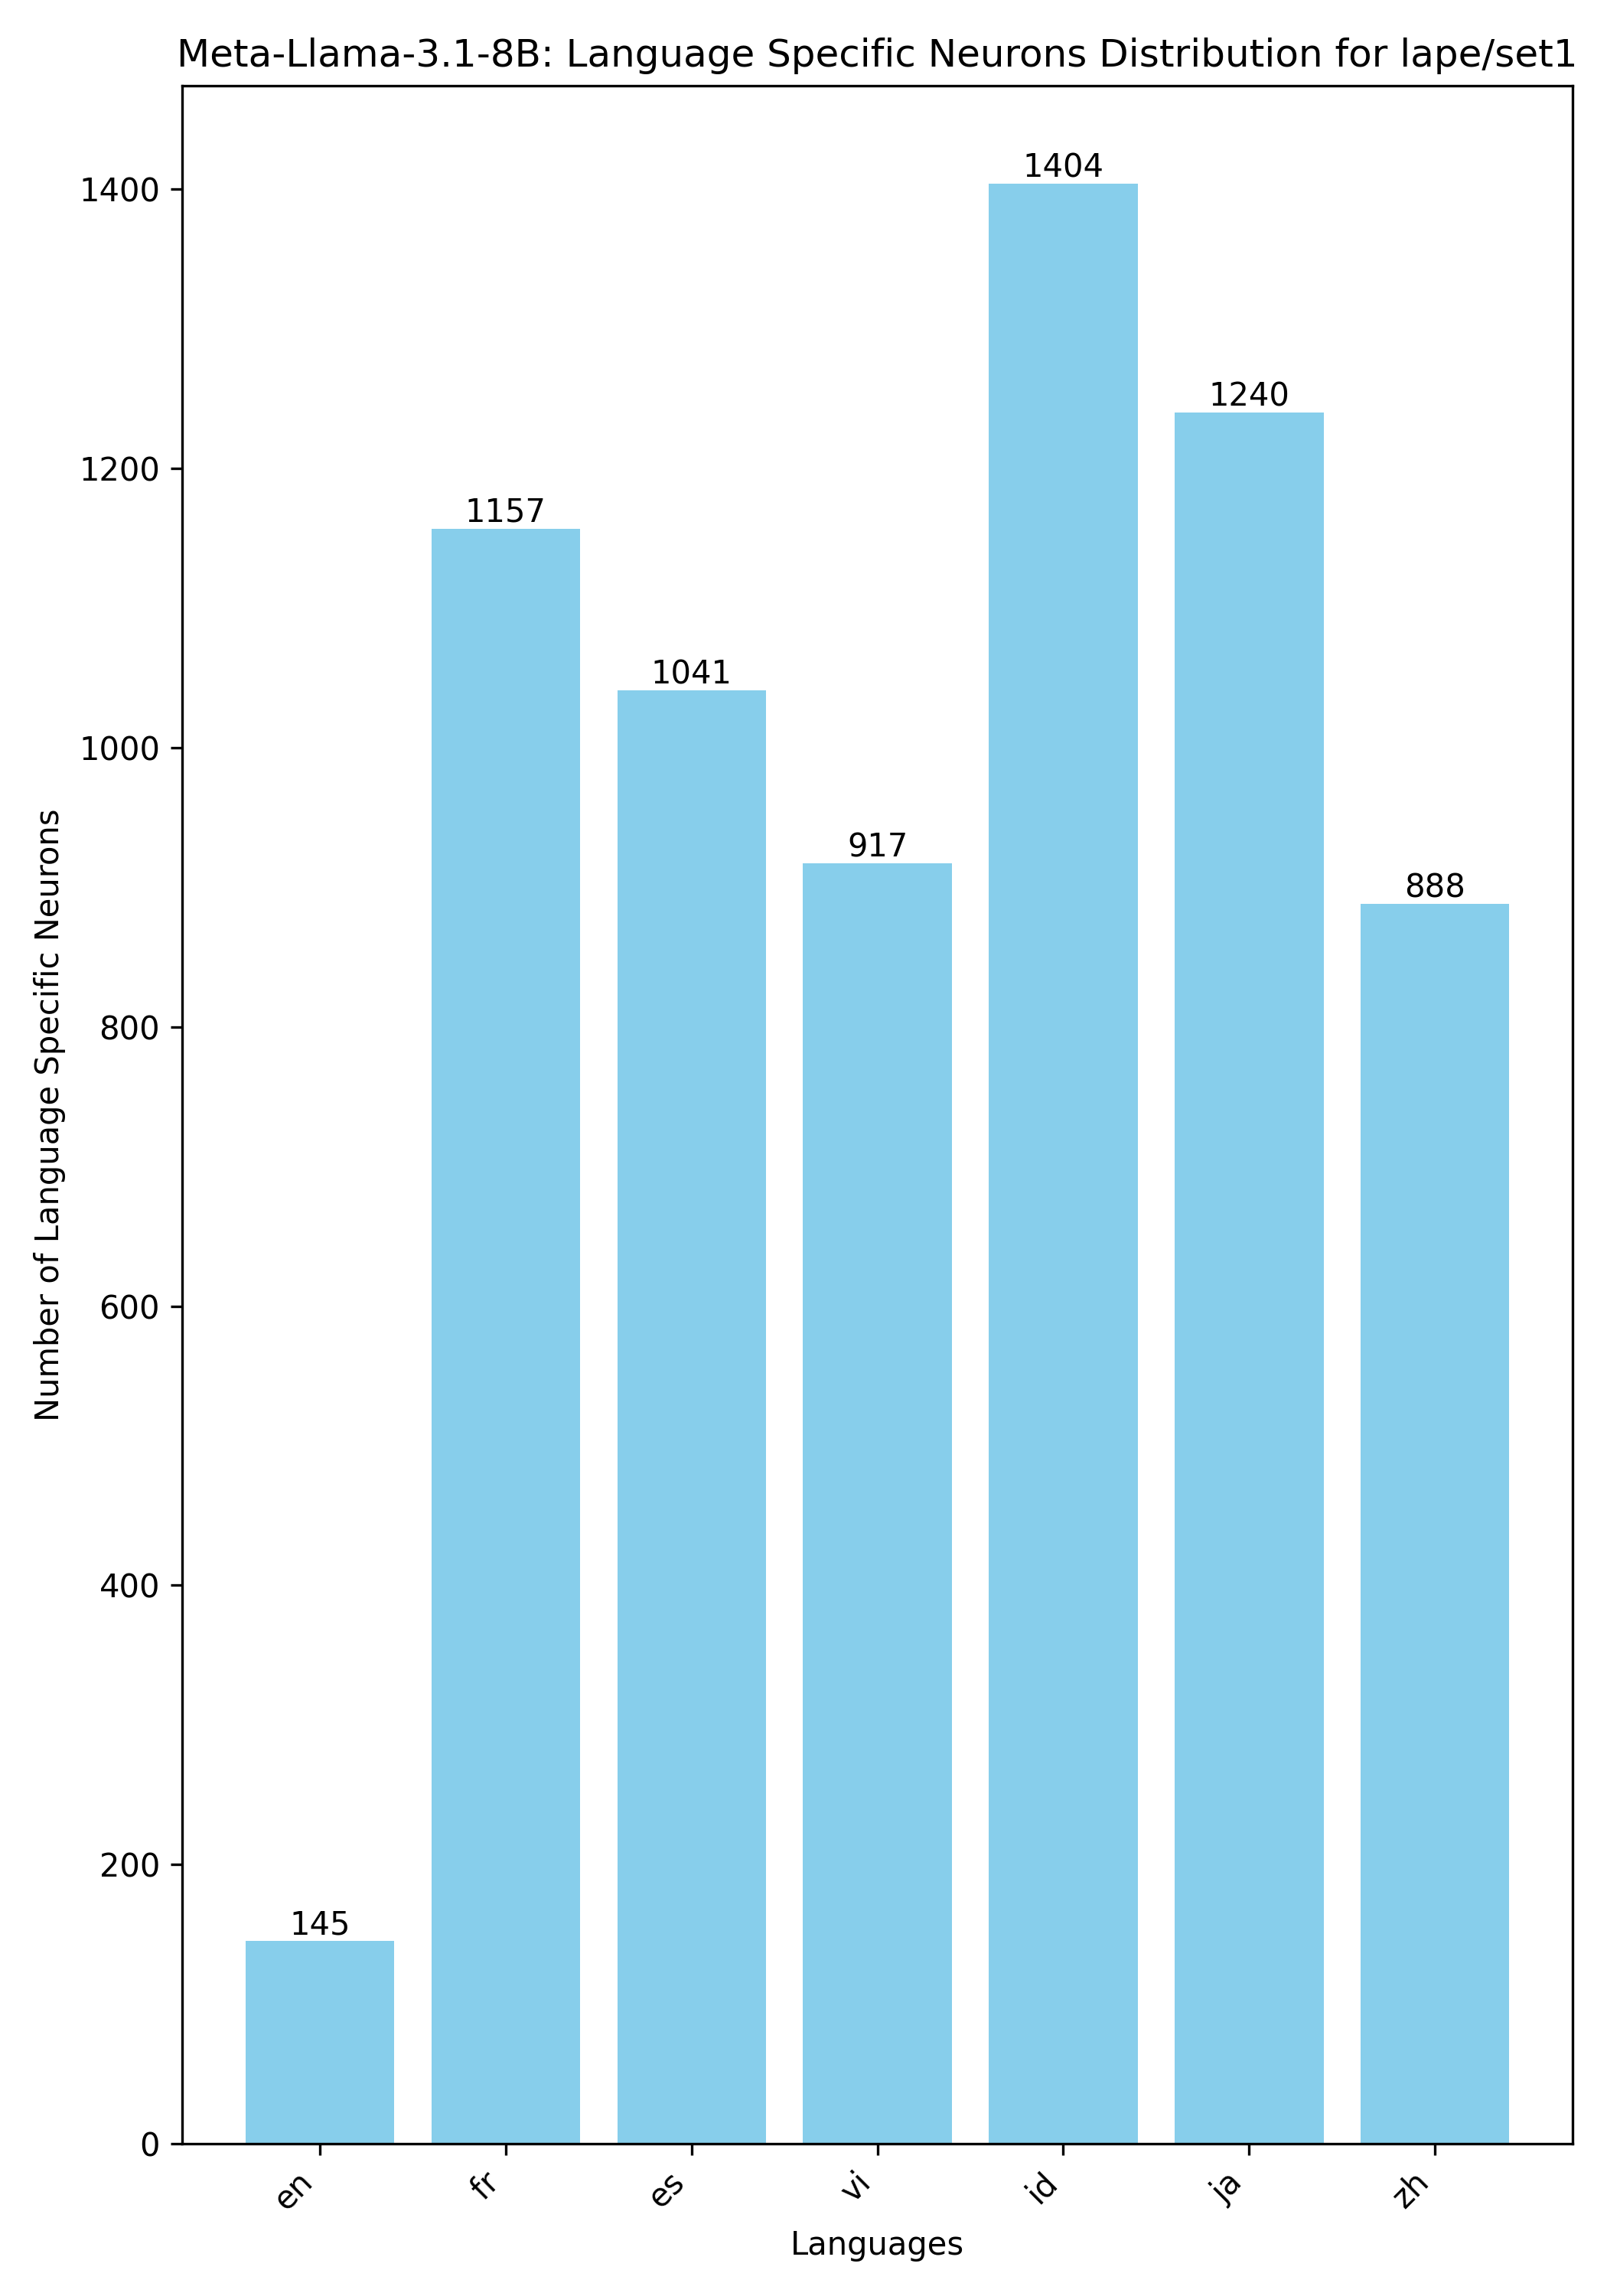
\includegraphics[width=0.45\textwidth]{Chapters/Chapter_5/lang_neurons/Meta-Llama-3.1-8B/lape/set1/lang_neuron_dist.png} &
		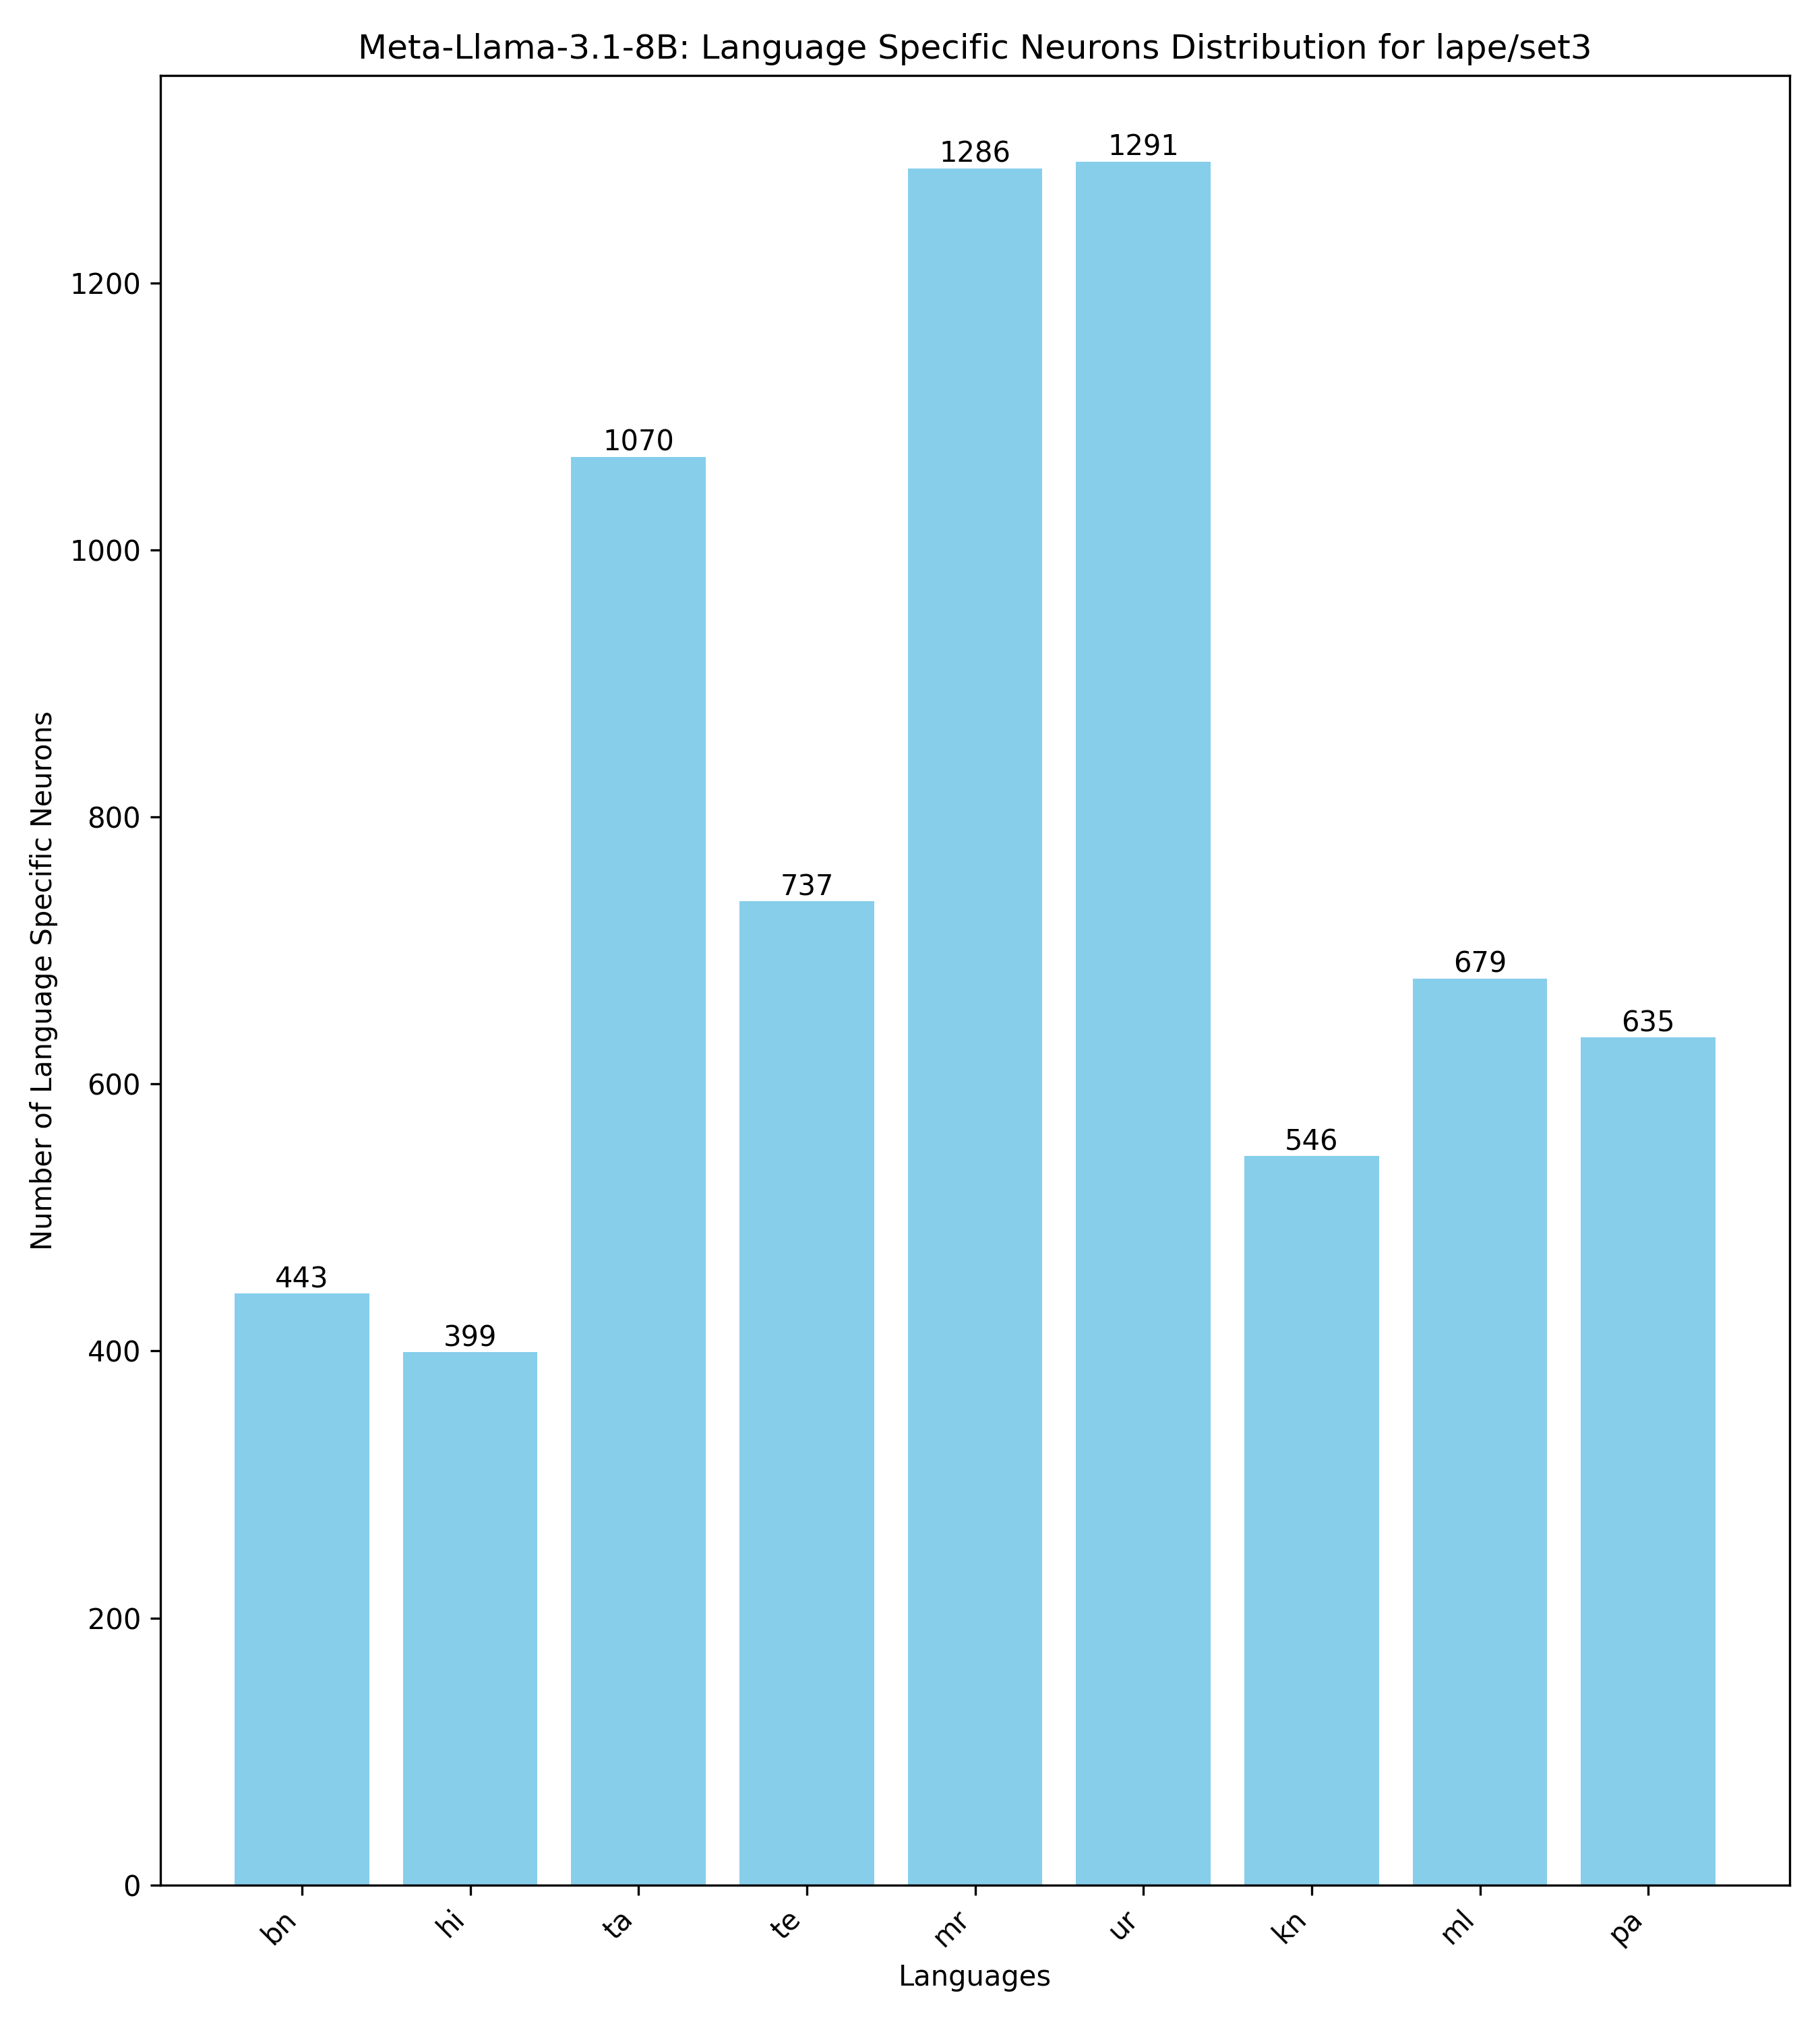
\includegraphics[width=0.45\textwidth]{Chapters/Chapter_5/lang_neurons/Meta-Llama-3.1-8B/lape/set3/lang_neuron_dist.png} \\
		\textbf{Set1: Language Neuron Distribution} &
		\textbf{Set3: Language Neuron Distribution}
	\end{tabular}
	\caption{Language-specific neuron distributions for LAPE method for Set1 and Set3.}
	\label{fig:lang_neuron_distribution}
\end{figure}

From Figure \ref{fig:lang_neuron_distribution}, it is evident that certain languages, such as \textit{id}, \textit{ja}, \textit{ur}, and \textit{mr}, have higher neuron counts, suggesting that the model dedicates more capacity to languages with rich morphology or syntactic structures. Conversely, \textit{en} consistently has the fewest neurons, likely due to its large amount of training data.

\textbf{Neuron Overlap Between Languages:} Figure \ref{fig:lang_neuron_overlap} illustrates the overlap of language-specific neurons between languages in Set1 and Set3. The overlap is formally calculated as:
\begin{equation}
	O_{l_1, l_2} = \sum_{i=1}^{L} \sum_{j=1}^{4d} \mathbb{I}\left(p_{i,j}^{l_1} > \text{Threshold}\right) \cdot \mathbb{I}\left(p_{i,j}^{l_2} > \text{Threshold}\right) \cdot \delta\left( (i,j) \in \text{Lang\_Set} \right),
\end{equation}
where $O_{l_1, l_2}$ represents the number of neurons shared between languages $l_1$ and $l_2$. 

\begin{figure}[ht]
	\centering
	\begin{tabular}{cc}
		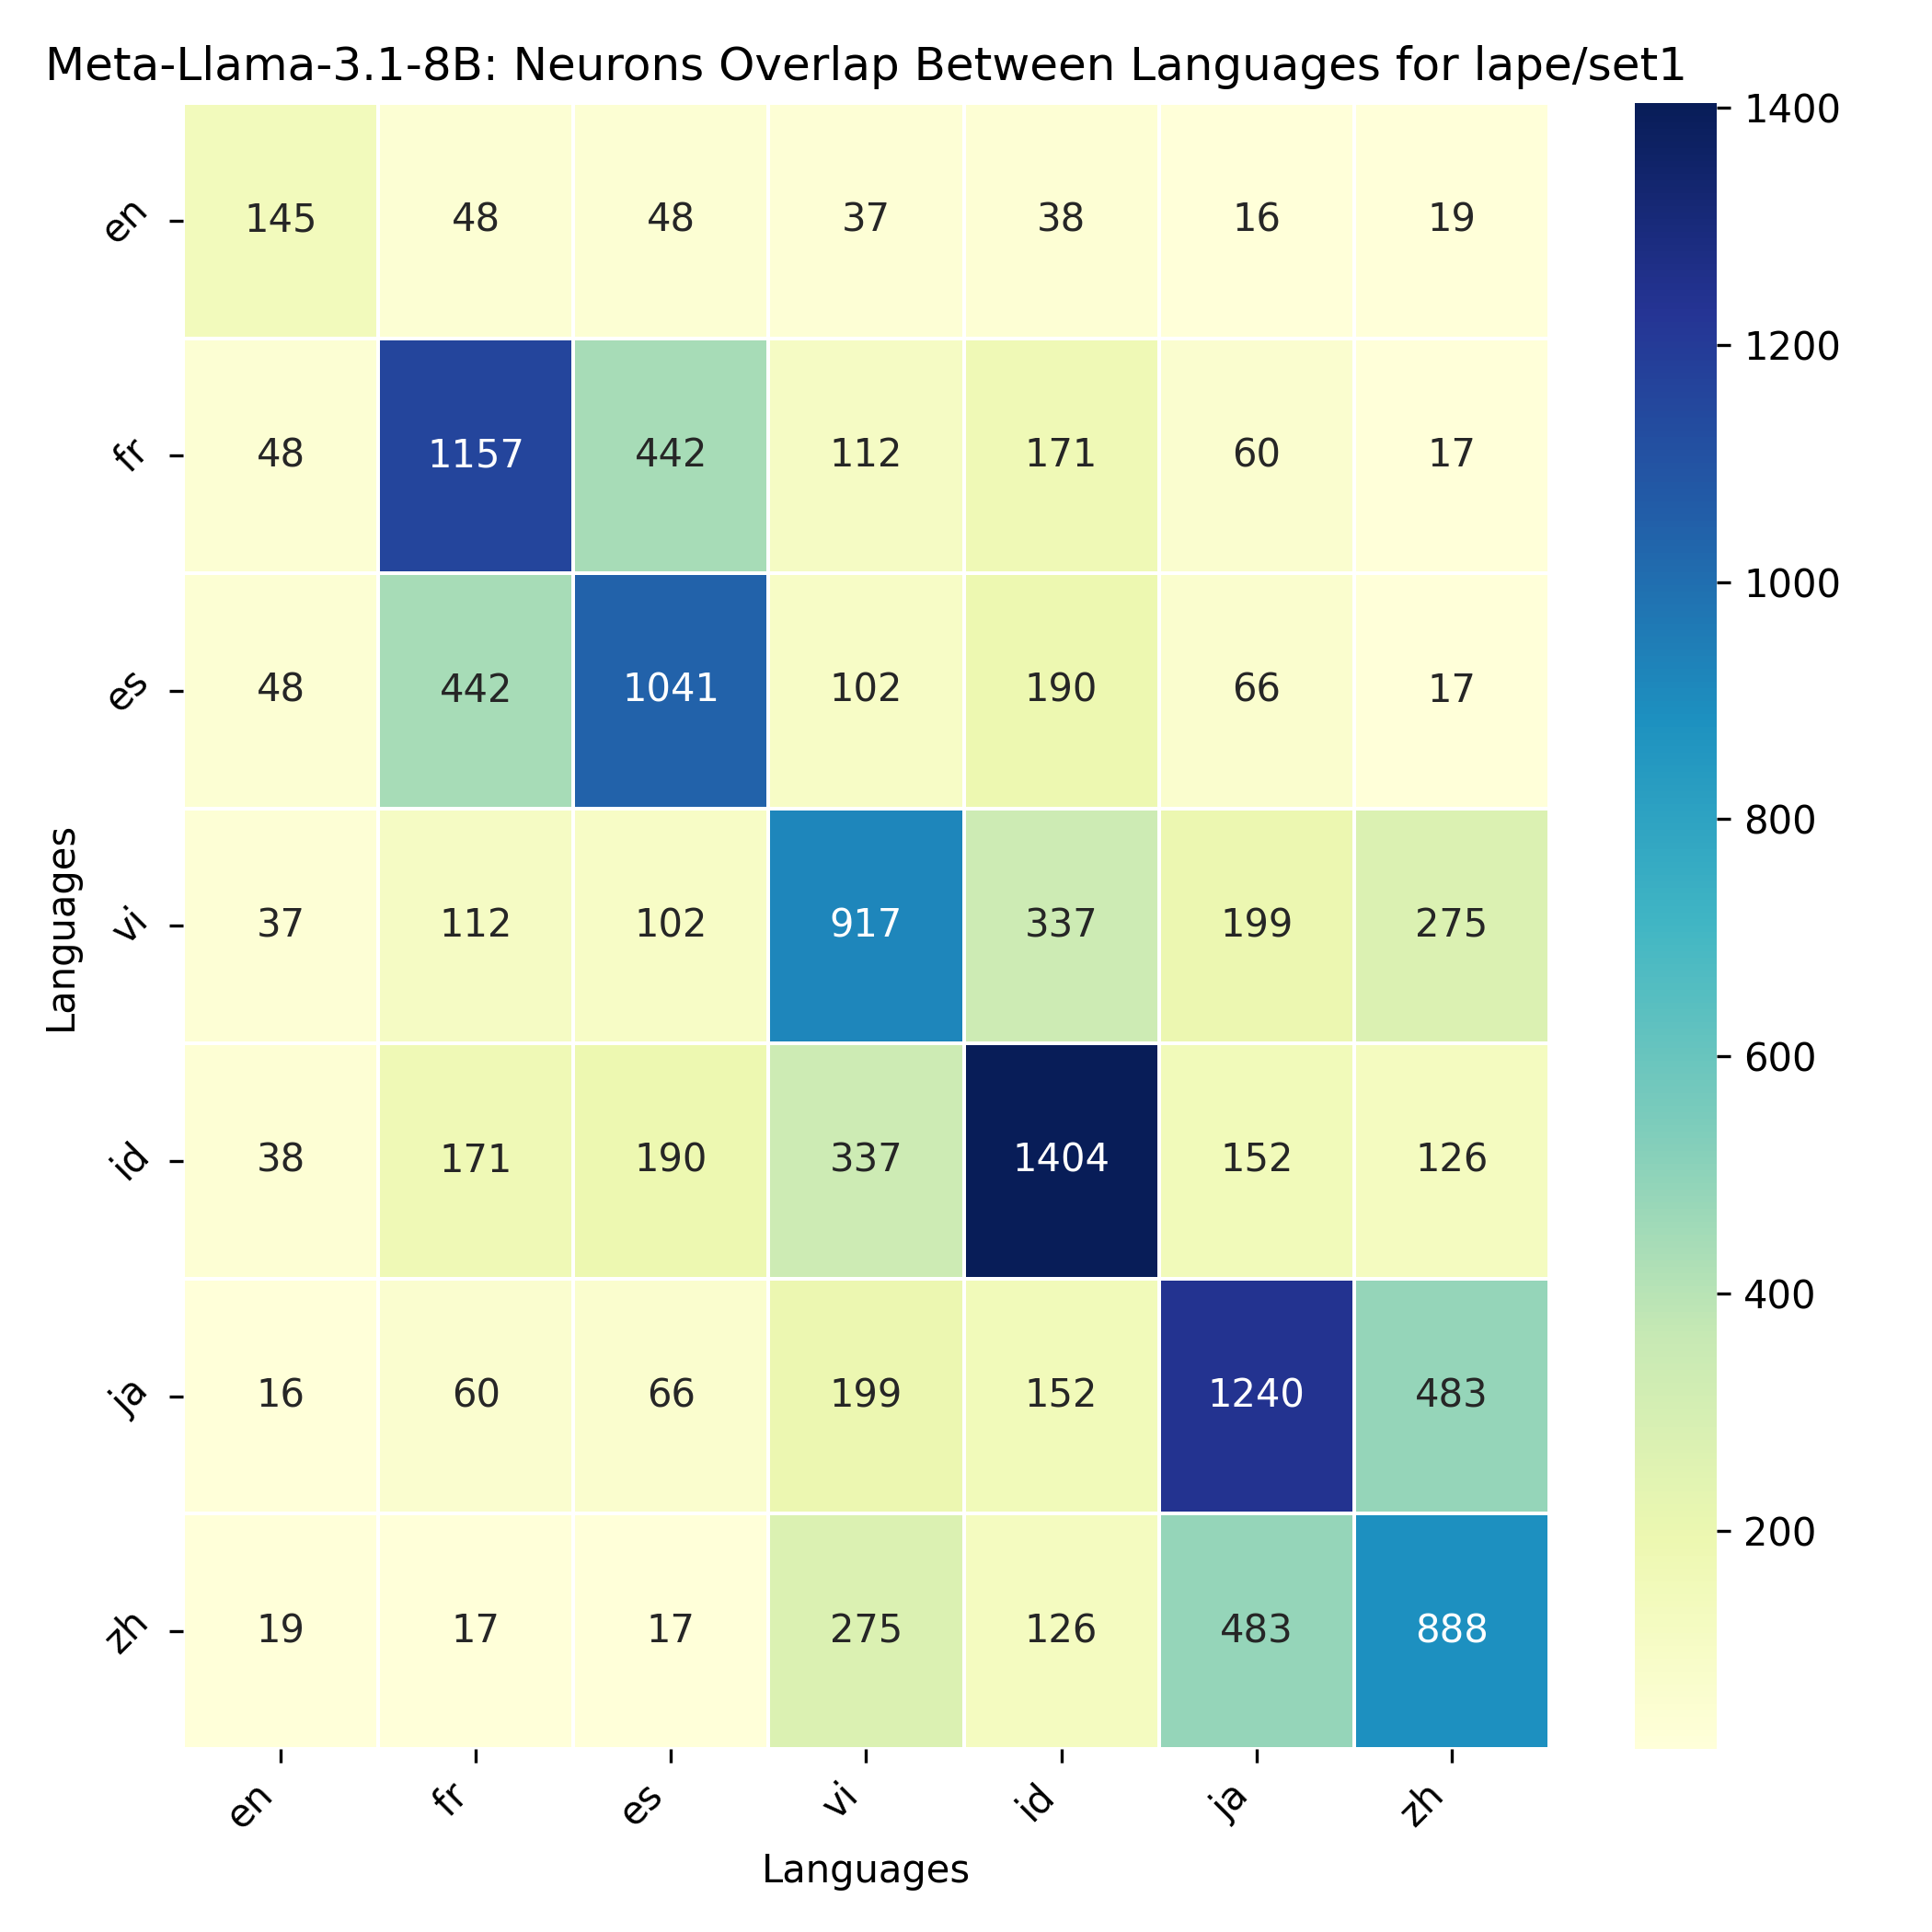
\includegraphics[width=0.45\textwidth]{Chapters/Chapter_5/lang_neurons/Meta-Llama-3.1-8B/lape/set1/lang_neurons_overlap.png} &
		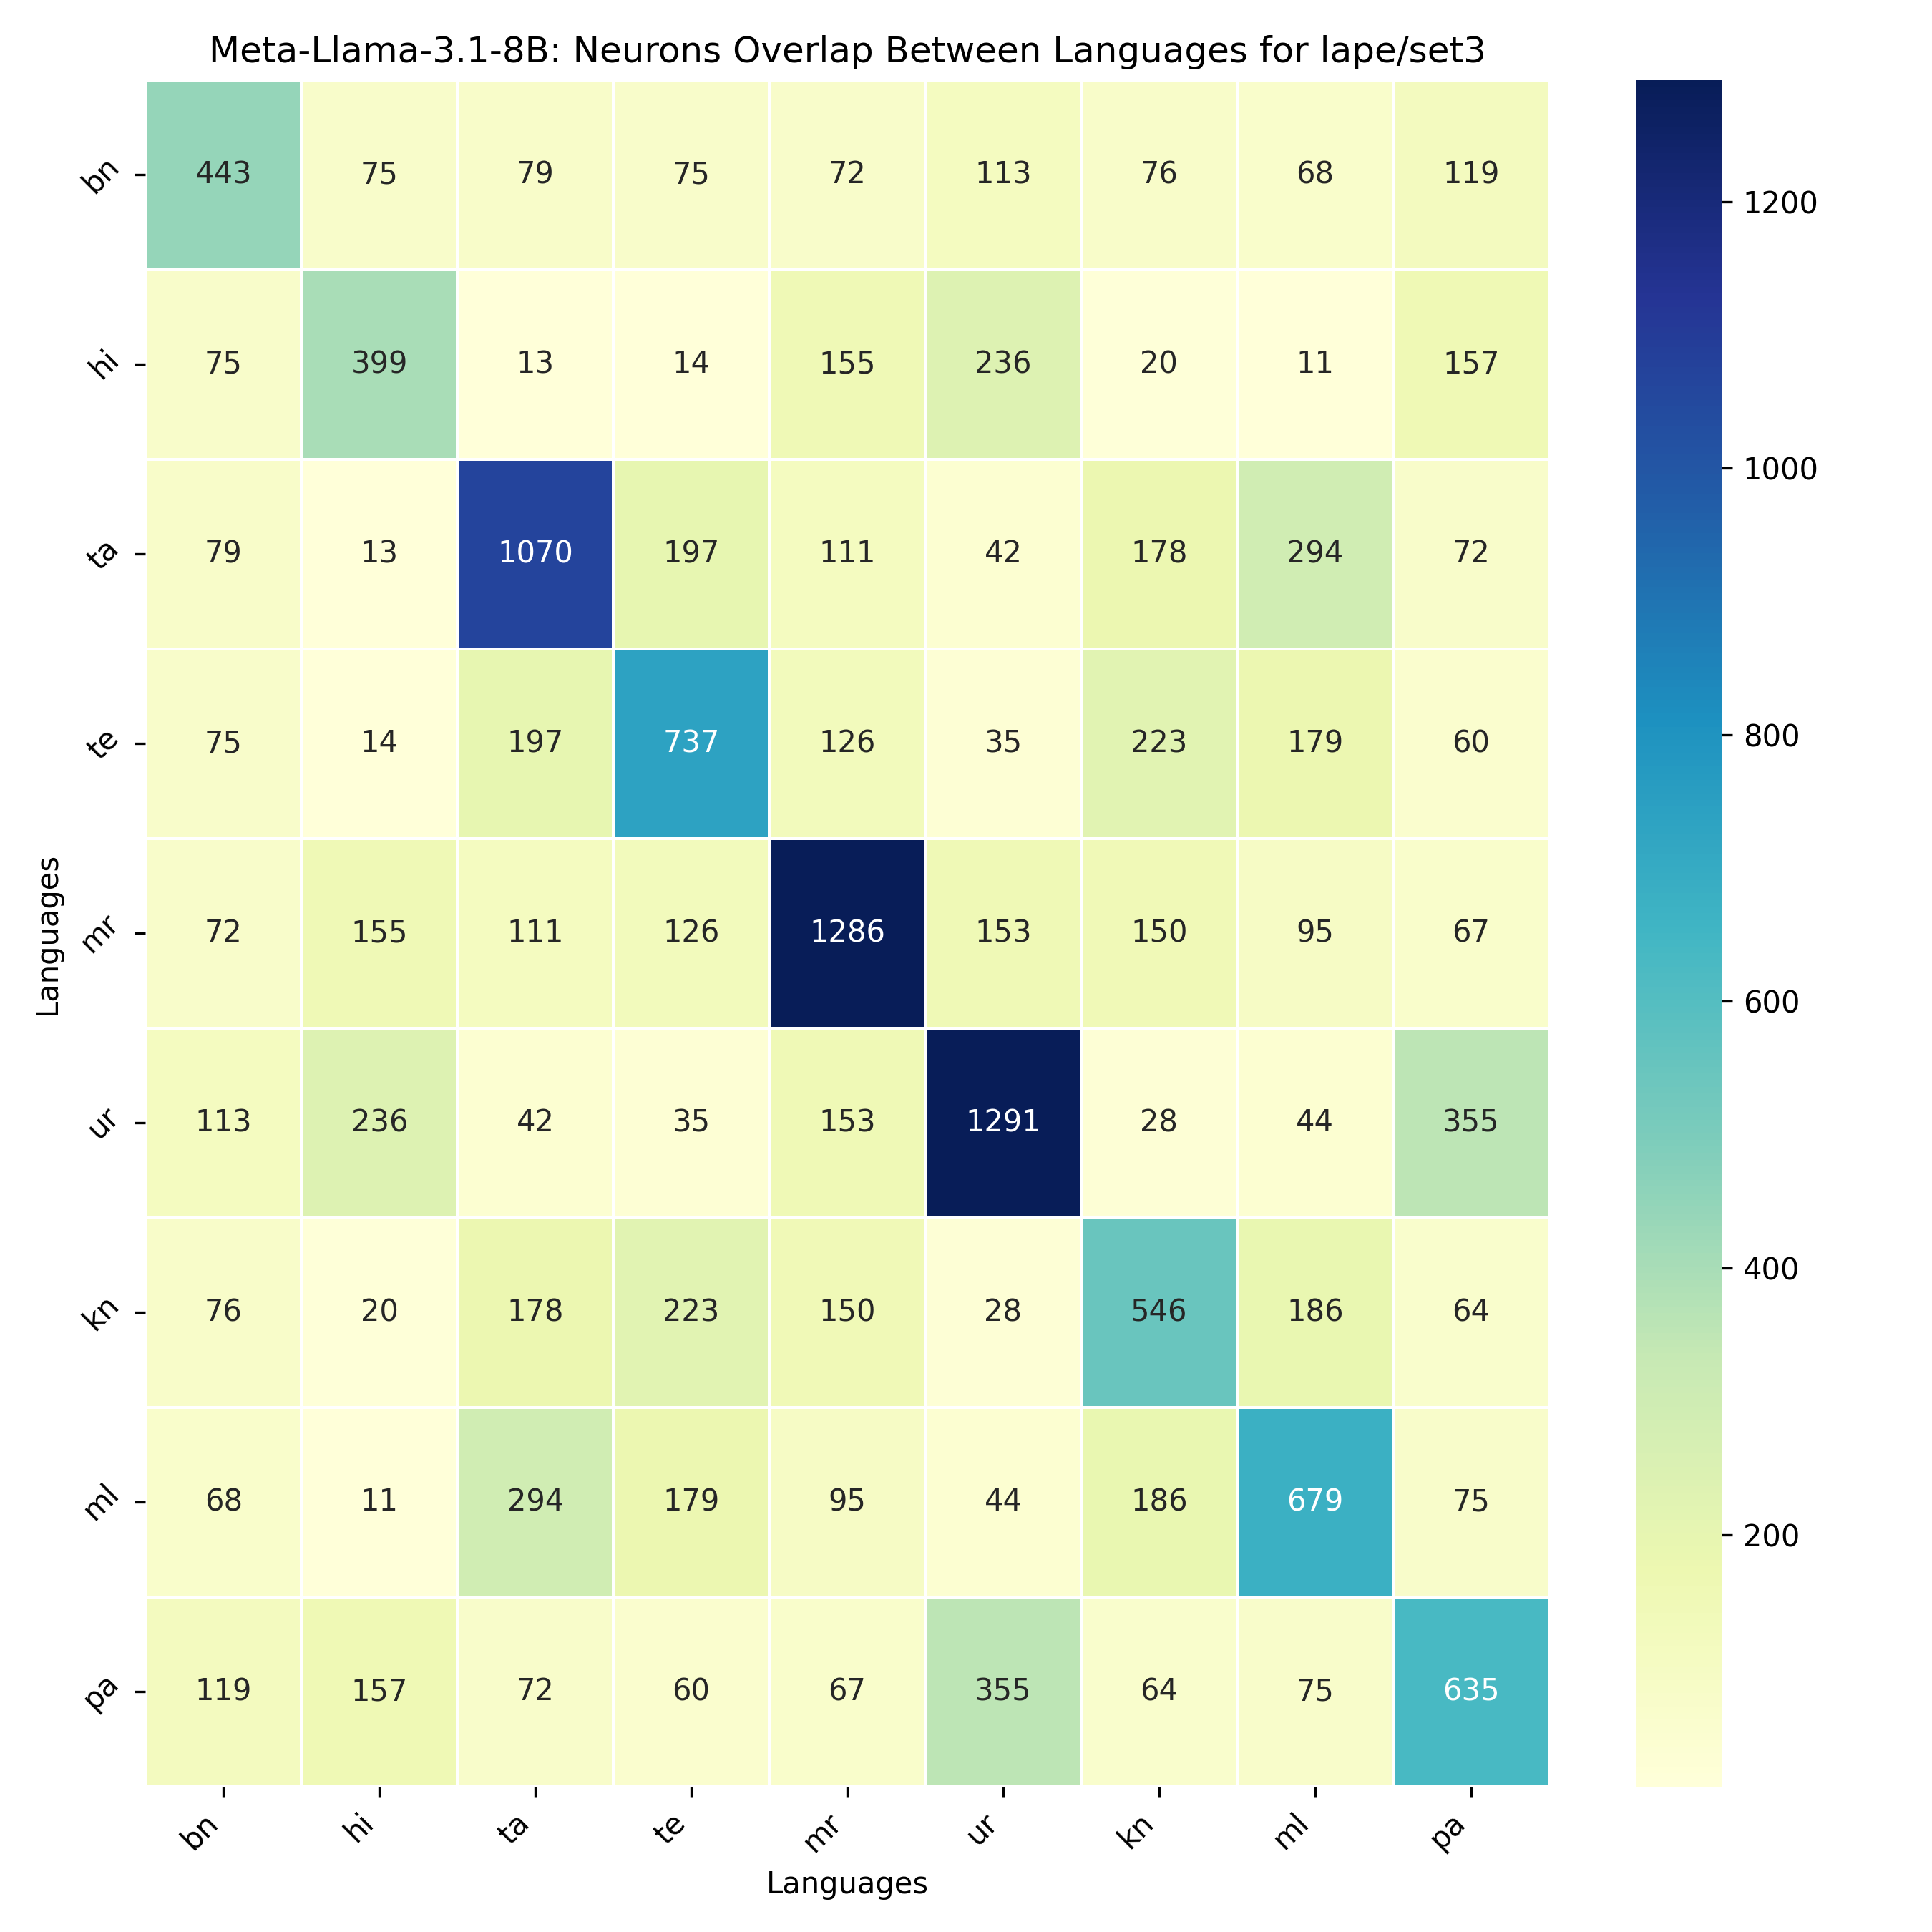
\includegraphics[width=0.45\textwidth]{Chapters/Chapter_5/lang_neurons/Meta-Llama-3.1-8B/lape/set3/lang_neurons_overlap.png} \\
		\textbf{Set1: Neuron Overlap} &
		\textbf{Set3: Neuron Overlap}
	\end{tabular}
	\caption{Neuron overlap between languages for LAPE method for Set1 and Set3.}
	\label{fig:lang_neuron_overlap}
\end{figure}

Figure \ref{fig:lang_neuron_overlap} highlights that languages with shared syntactic or morphological properties, such as \textit{id} and \textit{vi} in Set1, exhibit higher overlap. In contrast, languages like \textit{en} and \textit{fr} have minimal overlap with other languages, underscoring their unique linguistic structures.

\textbf{Layer-Wise Neuron Distribution:} The layer-wise distribution of language-specific neurons for Set1 and Set3 is shown in Figure \ref{fig:layerwise_distribution}. The distribution is computed as:
\begin{equation}
	L_l(i) = \sum_{j=1}^{4d} \mathbb{I}\left(p_{i,j}^l > \text{Threshold}\right) \cdot \delta\left((i,j) \in \text{Lang\_Set}\right),
\end{equation}
where $L_l(i)$ denotes the number of neurons in layer $i$ associated with language $l$.

\begin{figure}[ht]
	\centering
	\begin{tabular}{cc}
		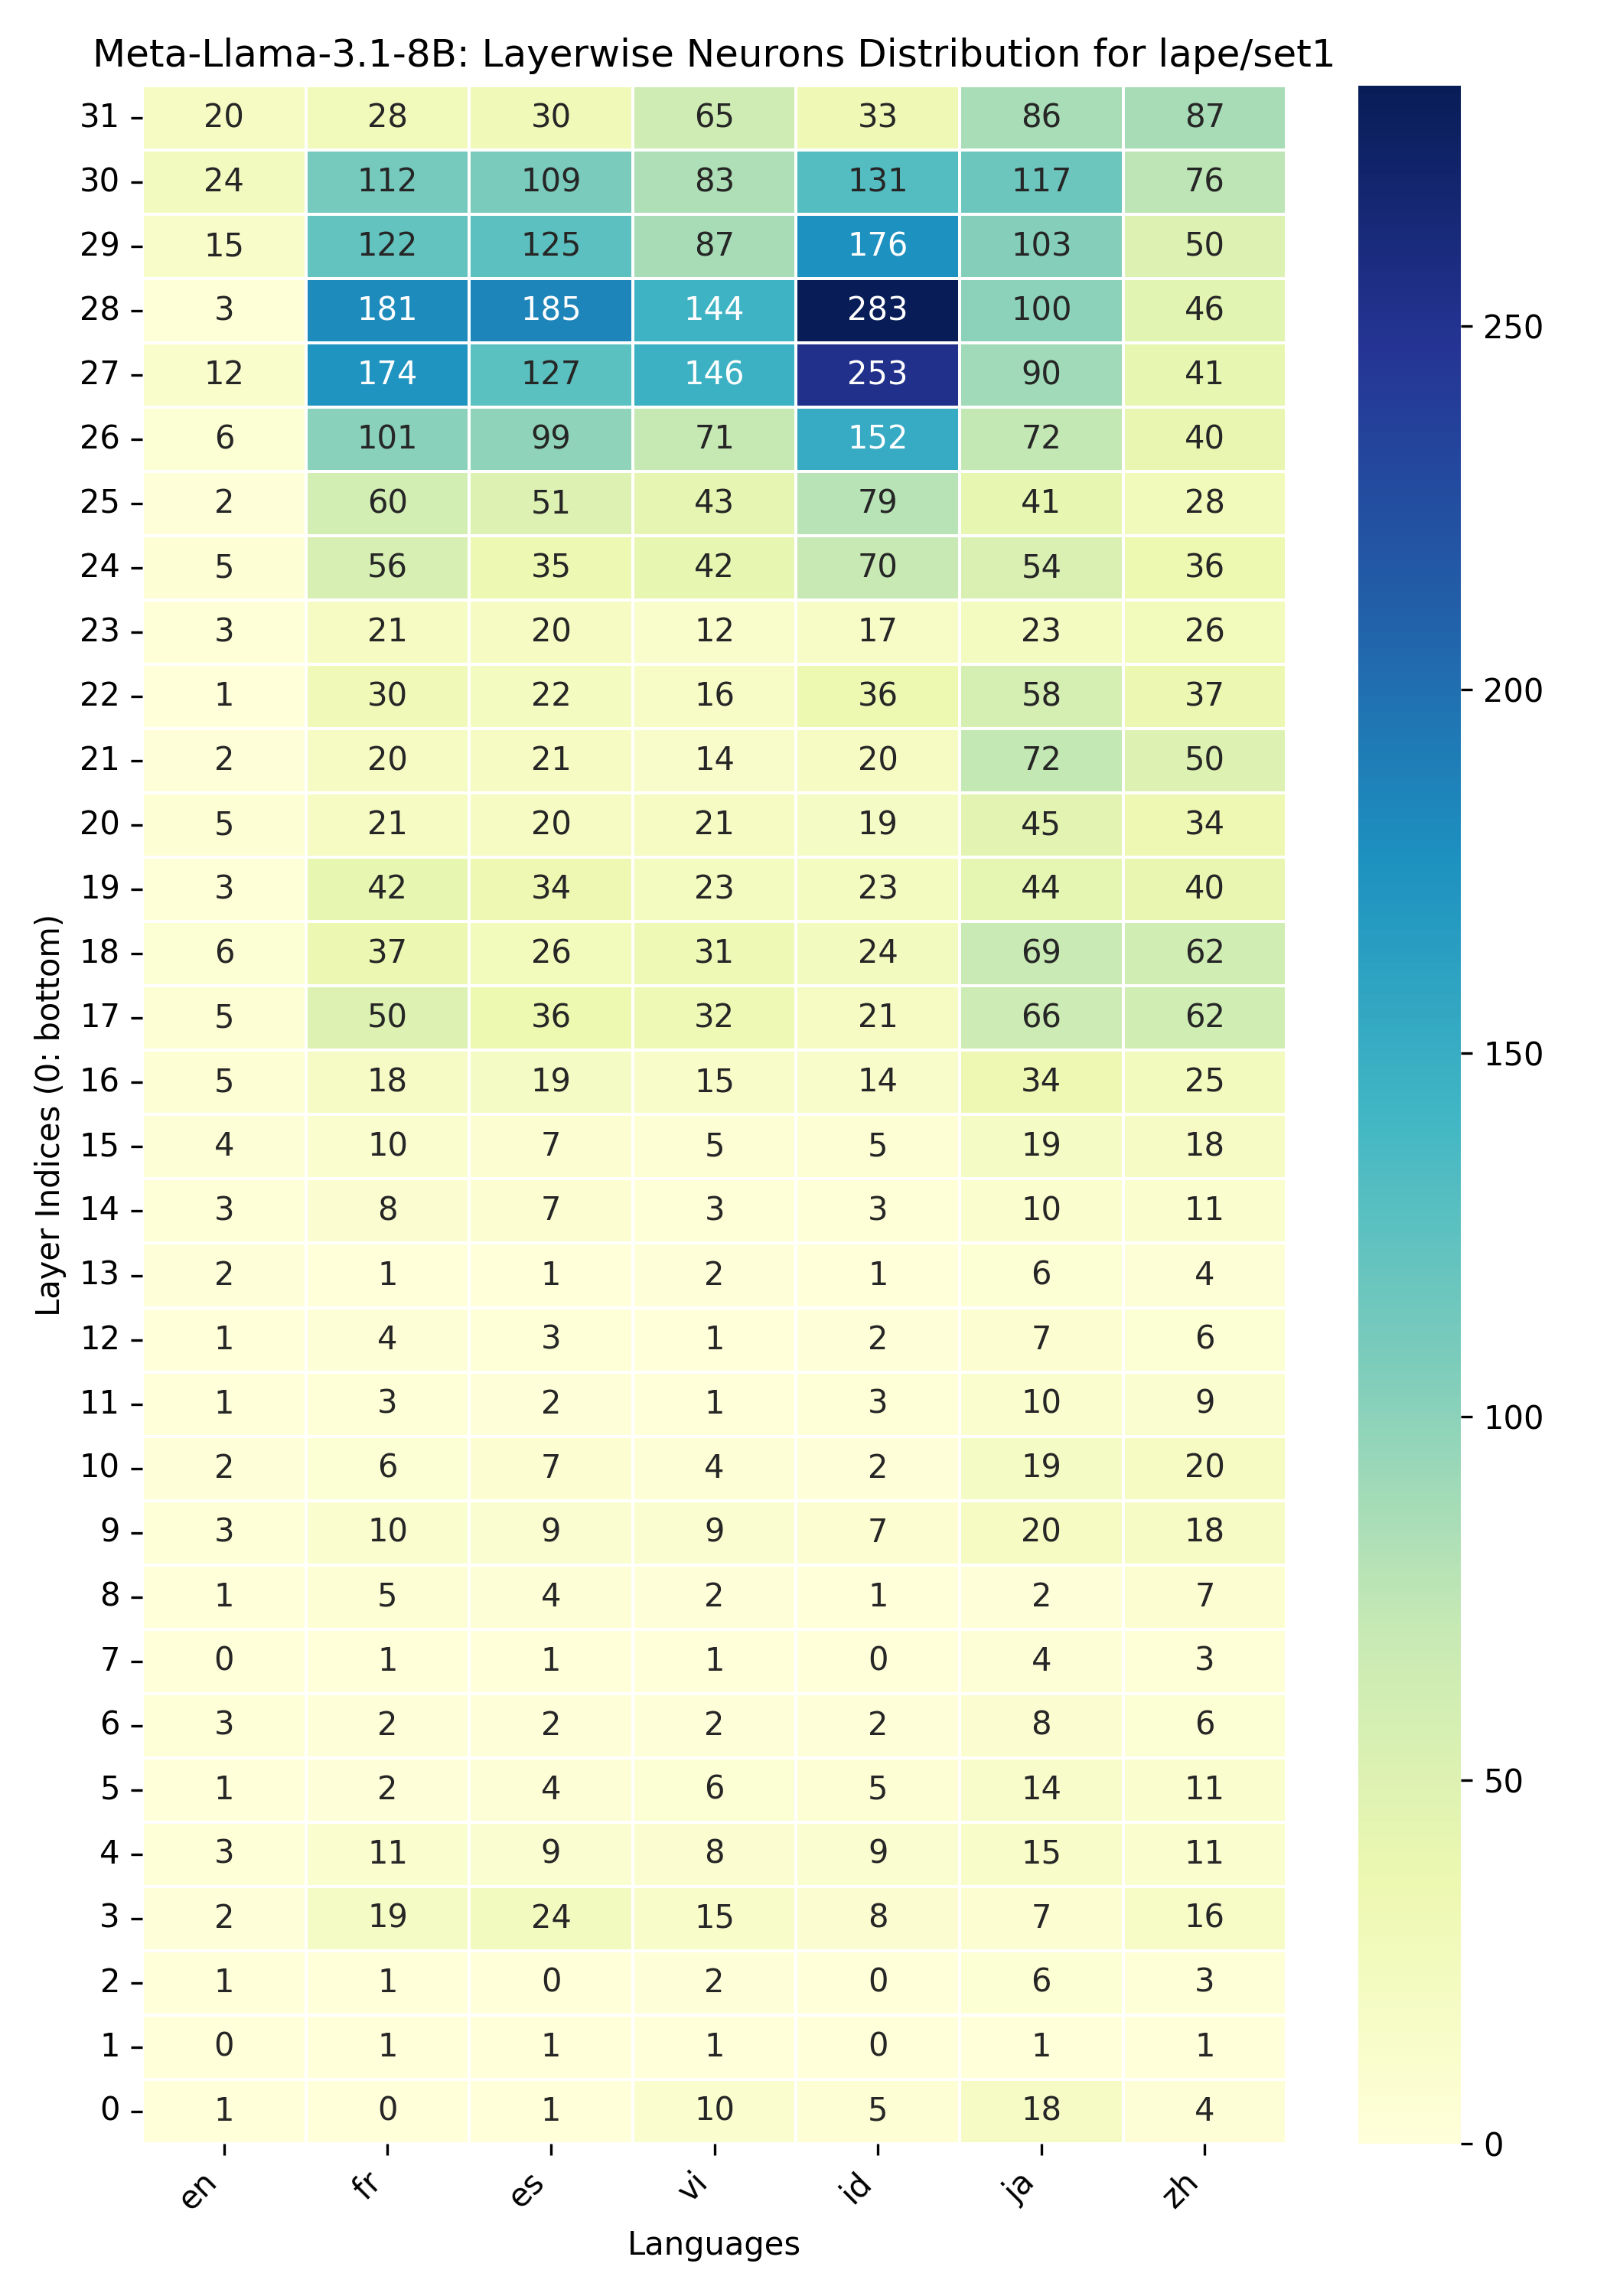
\includegraphics[width=0.45\textwidth]{Chapters/Chapter_5/lang_neurons/Meta-Llama-3.1-8B/lape/set1/layerwise_lang_neurons_dist.png} &
		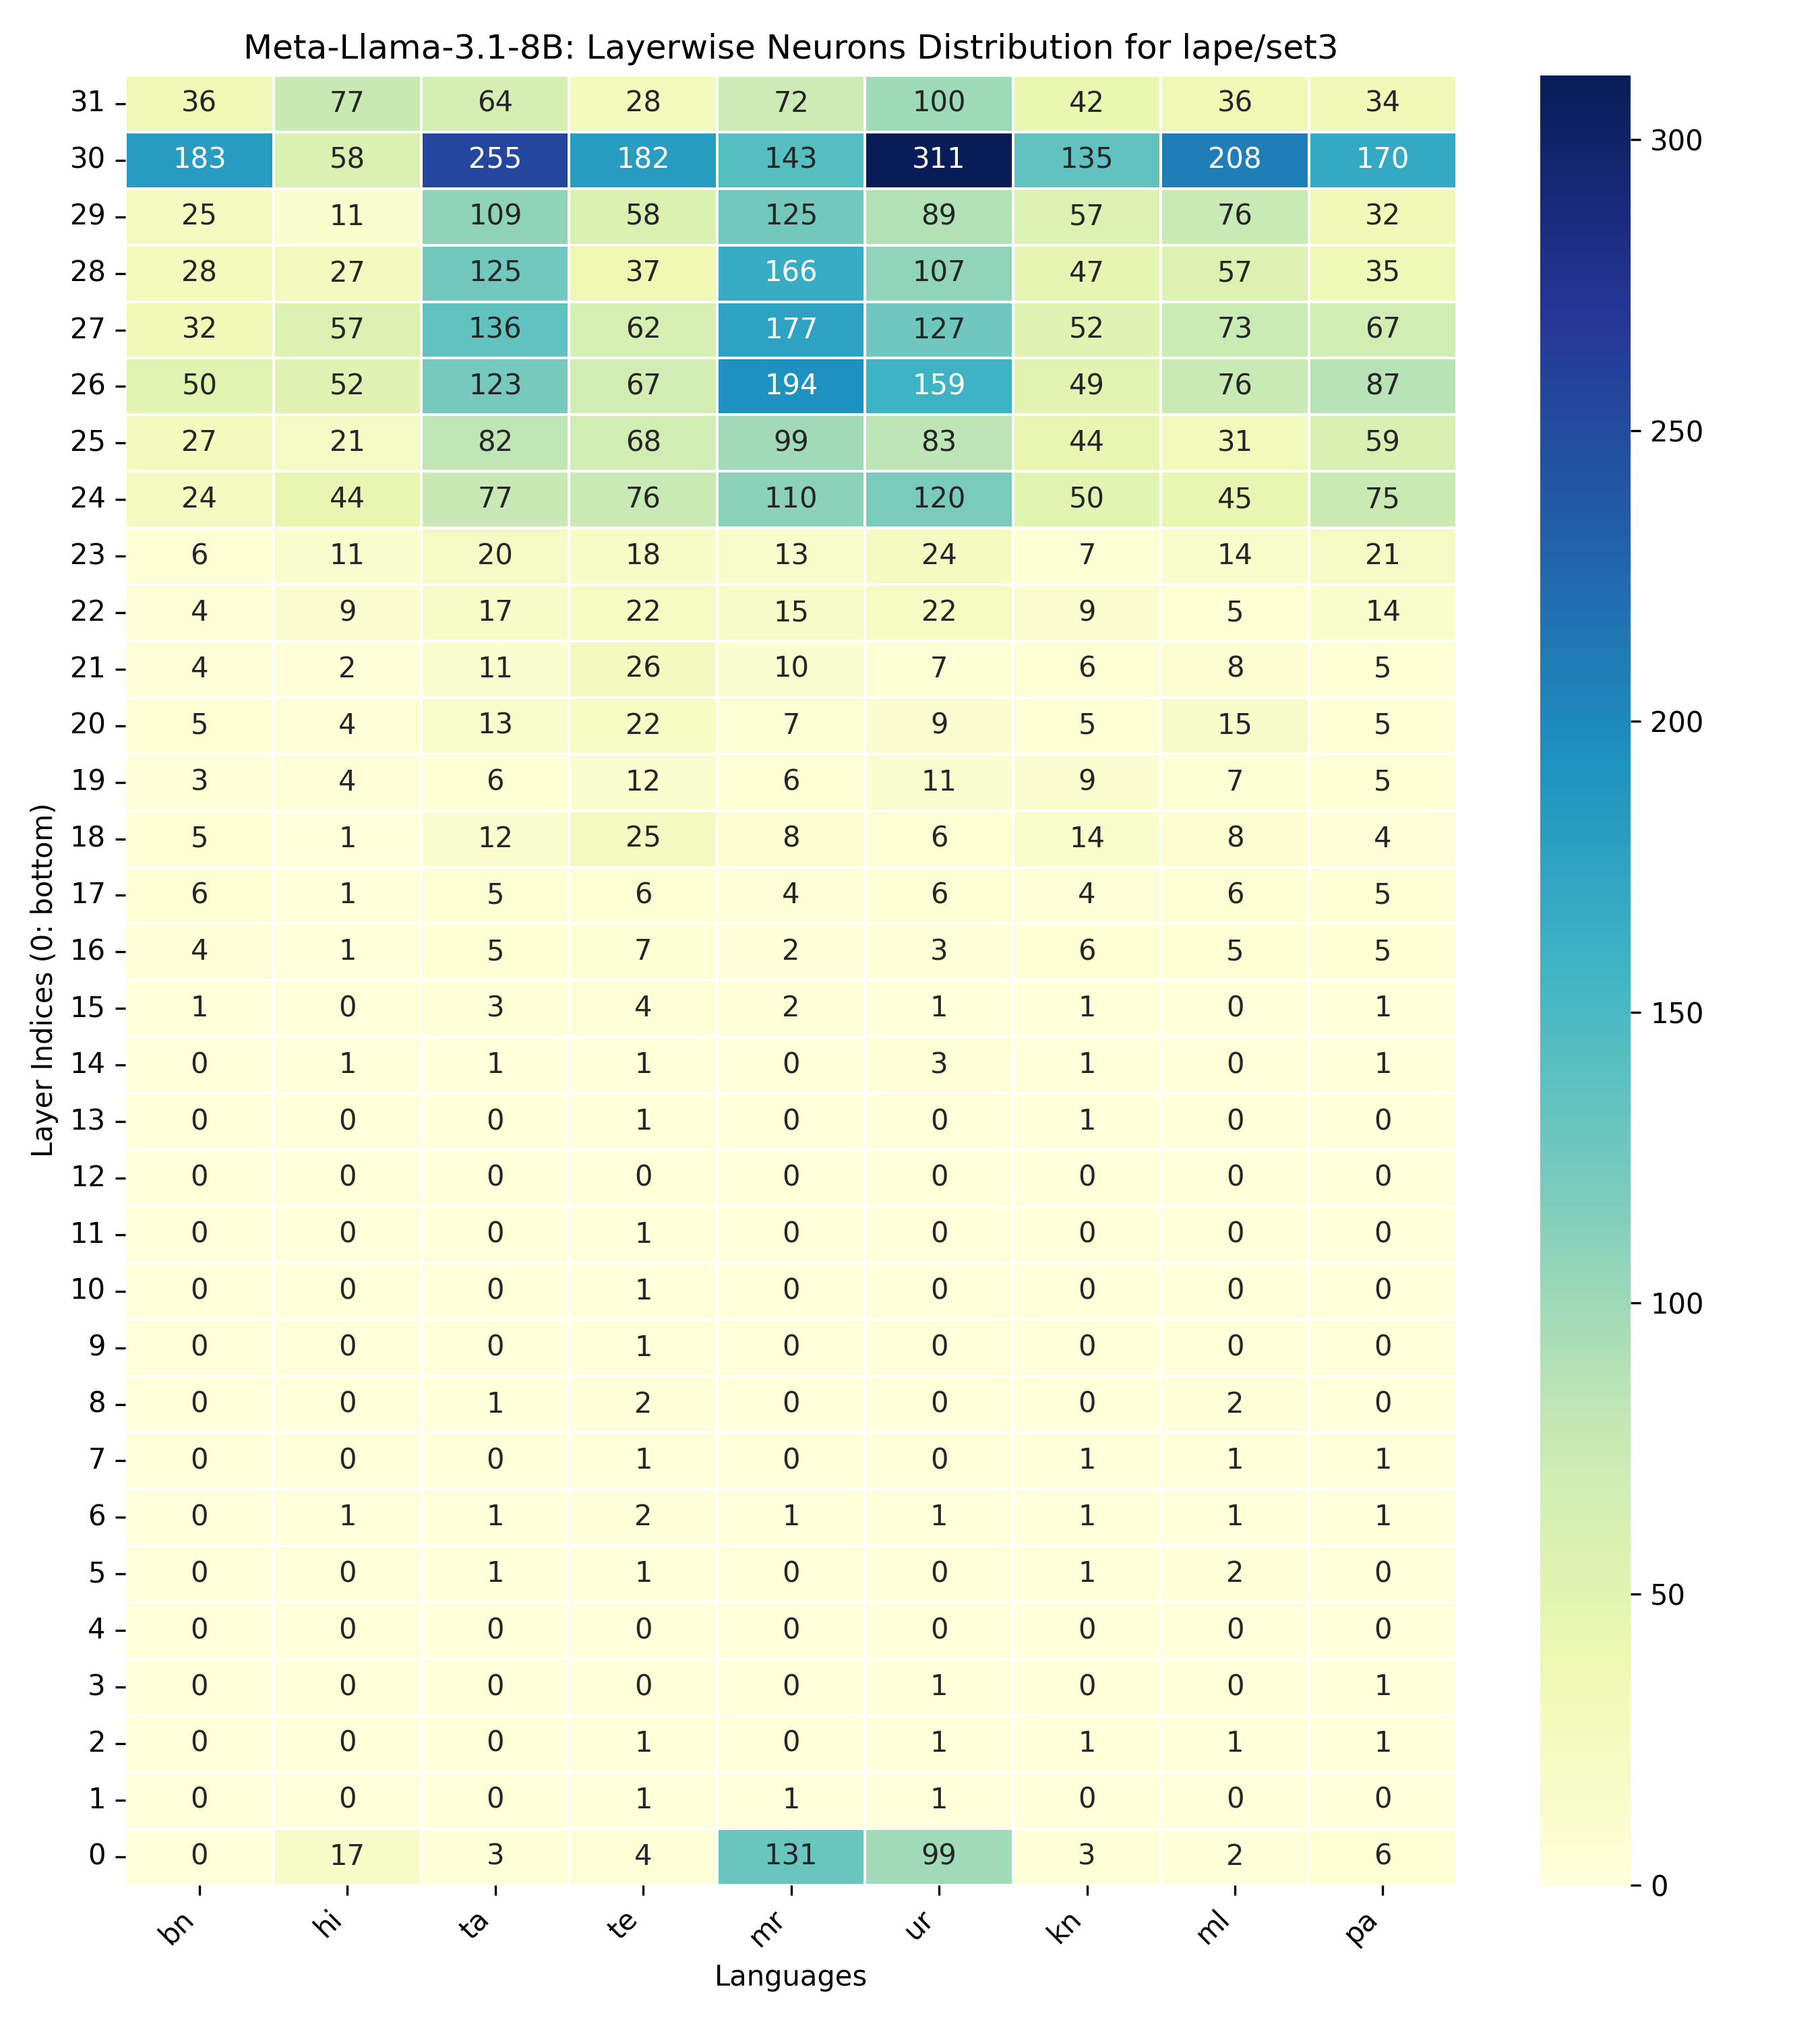
\includegraphics[width=0.45\textwidth]{Chapters/Chapter_5/lang_neurons/Meta-Llama-3.1-8B/lape/set3/layerwise_lang_neurons_dist.png} \\
		\textbf{Set1: Layer-wise Neuron Distribution} &
		\textbf{Set3: Layer-wise Neuron Distribution}
	\end{tabular}
	\caption{Layer-wise neuron distributions for LAPE method for Set1 and Set3.}
	\label{fig:layerwise_distribution}
\end{figure}

Figure \ref{fig:layerwise_distribution} reveals that language-specific neurons are concentrated in the upper layers (e.g., Layers 27-30), aligning with the notion that deeper layers capture more abstract and language-specific features. Lower layers exhibit fewer neurons, as they primarily encode shared linguistic features.

\subsection{Perplexity Change}

\textbf{Perplexity (PPX):} Perplexity is a widely used metric to evaluate the performance of language models. It measures how well a model predicts a sequence of tokens and is formally defined as the exponential of the average negative log-probability of the tokens in a sequence. 

Mathematically, for a sequence of tokens $\mathbf{x} = (x_1, x_2, \dots, x_T)$, the perplexity is given by:

\begin{equation}
	\text{PPX}(\mathbf{x}) = \exp\left(-\frac{1}{T} \sum_{t=1}^T \log P(x_t \,|\, x_{<t})\right),
\end{equation}

where:
\begin{itemize}
	\item $T$ is the length of the sequence.
	\item $P(x_t \,|\, x_{<t})$ is the probability assigned by the model to the token $x_t$, given the preceding tokens $x_{<t} = (x_1, x_2, \dots, x_{t-1})$.
\end{itemize}

Perplexity can be understood as the average branching factor of the model in predicting tokens. A lower perplexity indicates that the model is more confident in its predictions, while a higher perplexity suggests greater uncertainty.

For a dataset $\mathcal{D}$ consisting of multiple sequences, the perplexity is computed as the mean of the per-sequence perplexities:

\begin{equation}
	\text{PPX}(\mathcal{D}) = \exp\left(-\frac{1}{N} \sum_{i=1}^N \frac{1}{T_i} \sum_{t=1}^{T_i} \log P(x_t^{(i)} \,|\, x_{<t}^{(i)})\right),
\end{equation}

where $N$ is the total number of sequences in the dataset, and $T_i$ is the length of the $i$-th sequence.

\textbf{Perplexity Change (PPXC):} In the context of language modeling, perplexity serves as a key metric to measure the performance of a model. It quantifies how well a probability distribution predicts a sample. The perplexity change $\text{PPXC}(i,j)$ measures the change in perplexity for a target language $j$ when an intervention is applied at a source language $i$. Formally, it is defined as:

\begin{equation}
	\text{PPXC}(i,j) = \text{PPX}(j \,|\, \text{Intervention at } i) - \text{PPX}(j),
\end{equation}

where $\text{PPX}(j)$ denotes the original perplexity for language $j$, and $\text{PPX}(j \,|\, \text{Intervention at } i)$ is the perplexity after performing an intervention at language $i$. Lower values of $\text{PPXC}(i,j)$ indicate minimal interference, whereas higher values highlight a significant change in the model's understanding of language $j$ due to the intervention.

\textbf{Experimental Setup:} For this experiment, we used the Wikipedia dataset for each language. The experiments were conducted for two sets of languages: \textbf{Set1}, containing \{\textit{en, fr, es, vi, id, ja, zh}\}, and \textbf{Set3}, containing \{\textit{bn, hi, ta, te, mr, ur, kn, ml, pa}\}. The perplexity values were computed for each language, both with and without intervention at other languages.

\textbf{Analysis:} The Figure \ref{fig:ppx_change} illustrates the perplexity changes for Set1 and Set3. Each heatmap represents $\text{PPXC}(i,j)$ values for different combinations of source and target languages. In all the experiments, the intervention means the values for the neuron activation is set as zero.

\begin{figure}[ht]
	\centering
	\begin{tabular}{cc}
		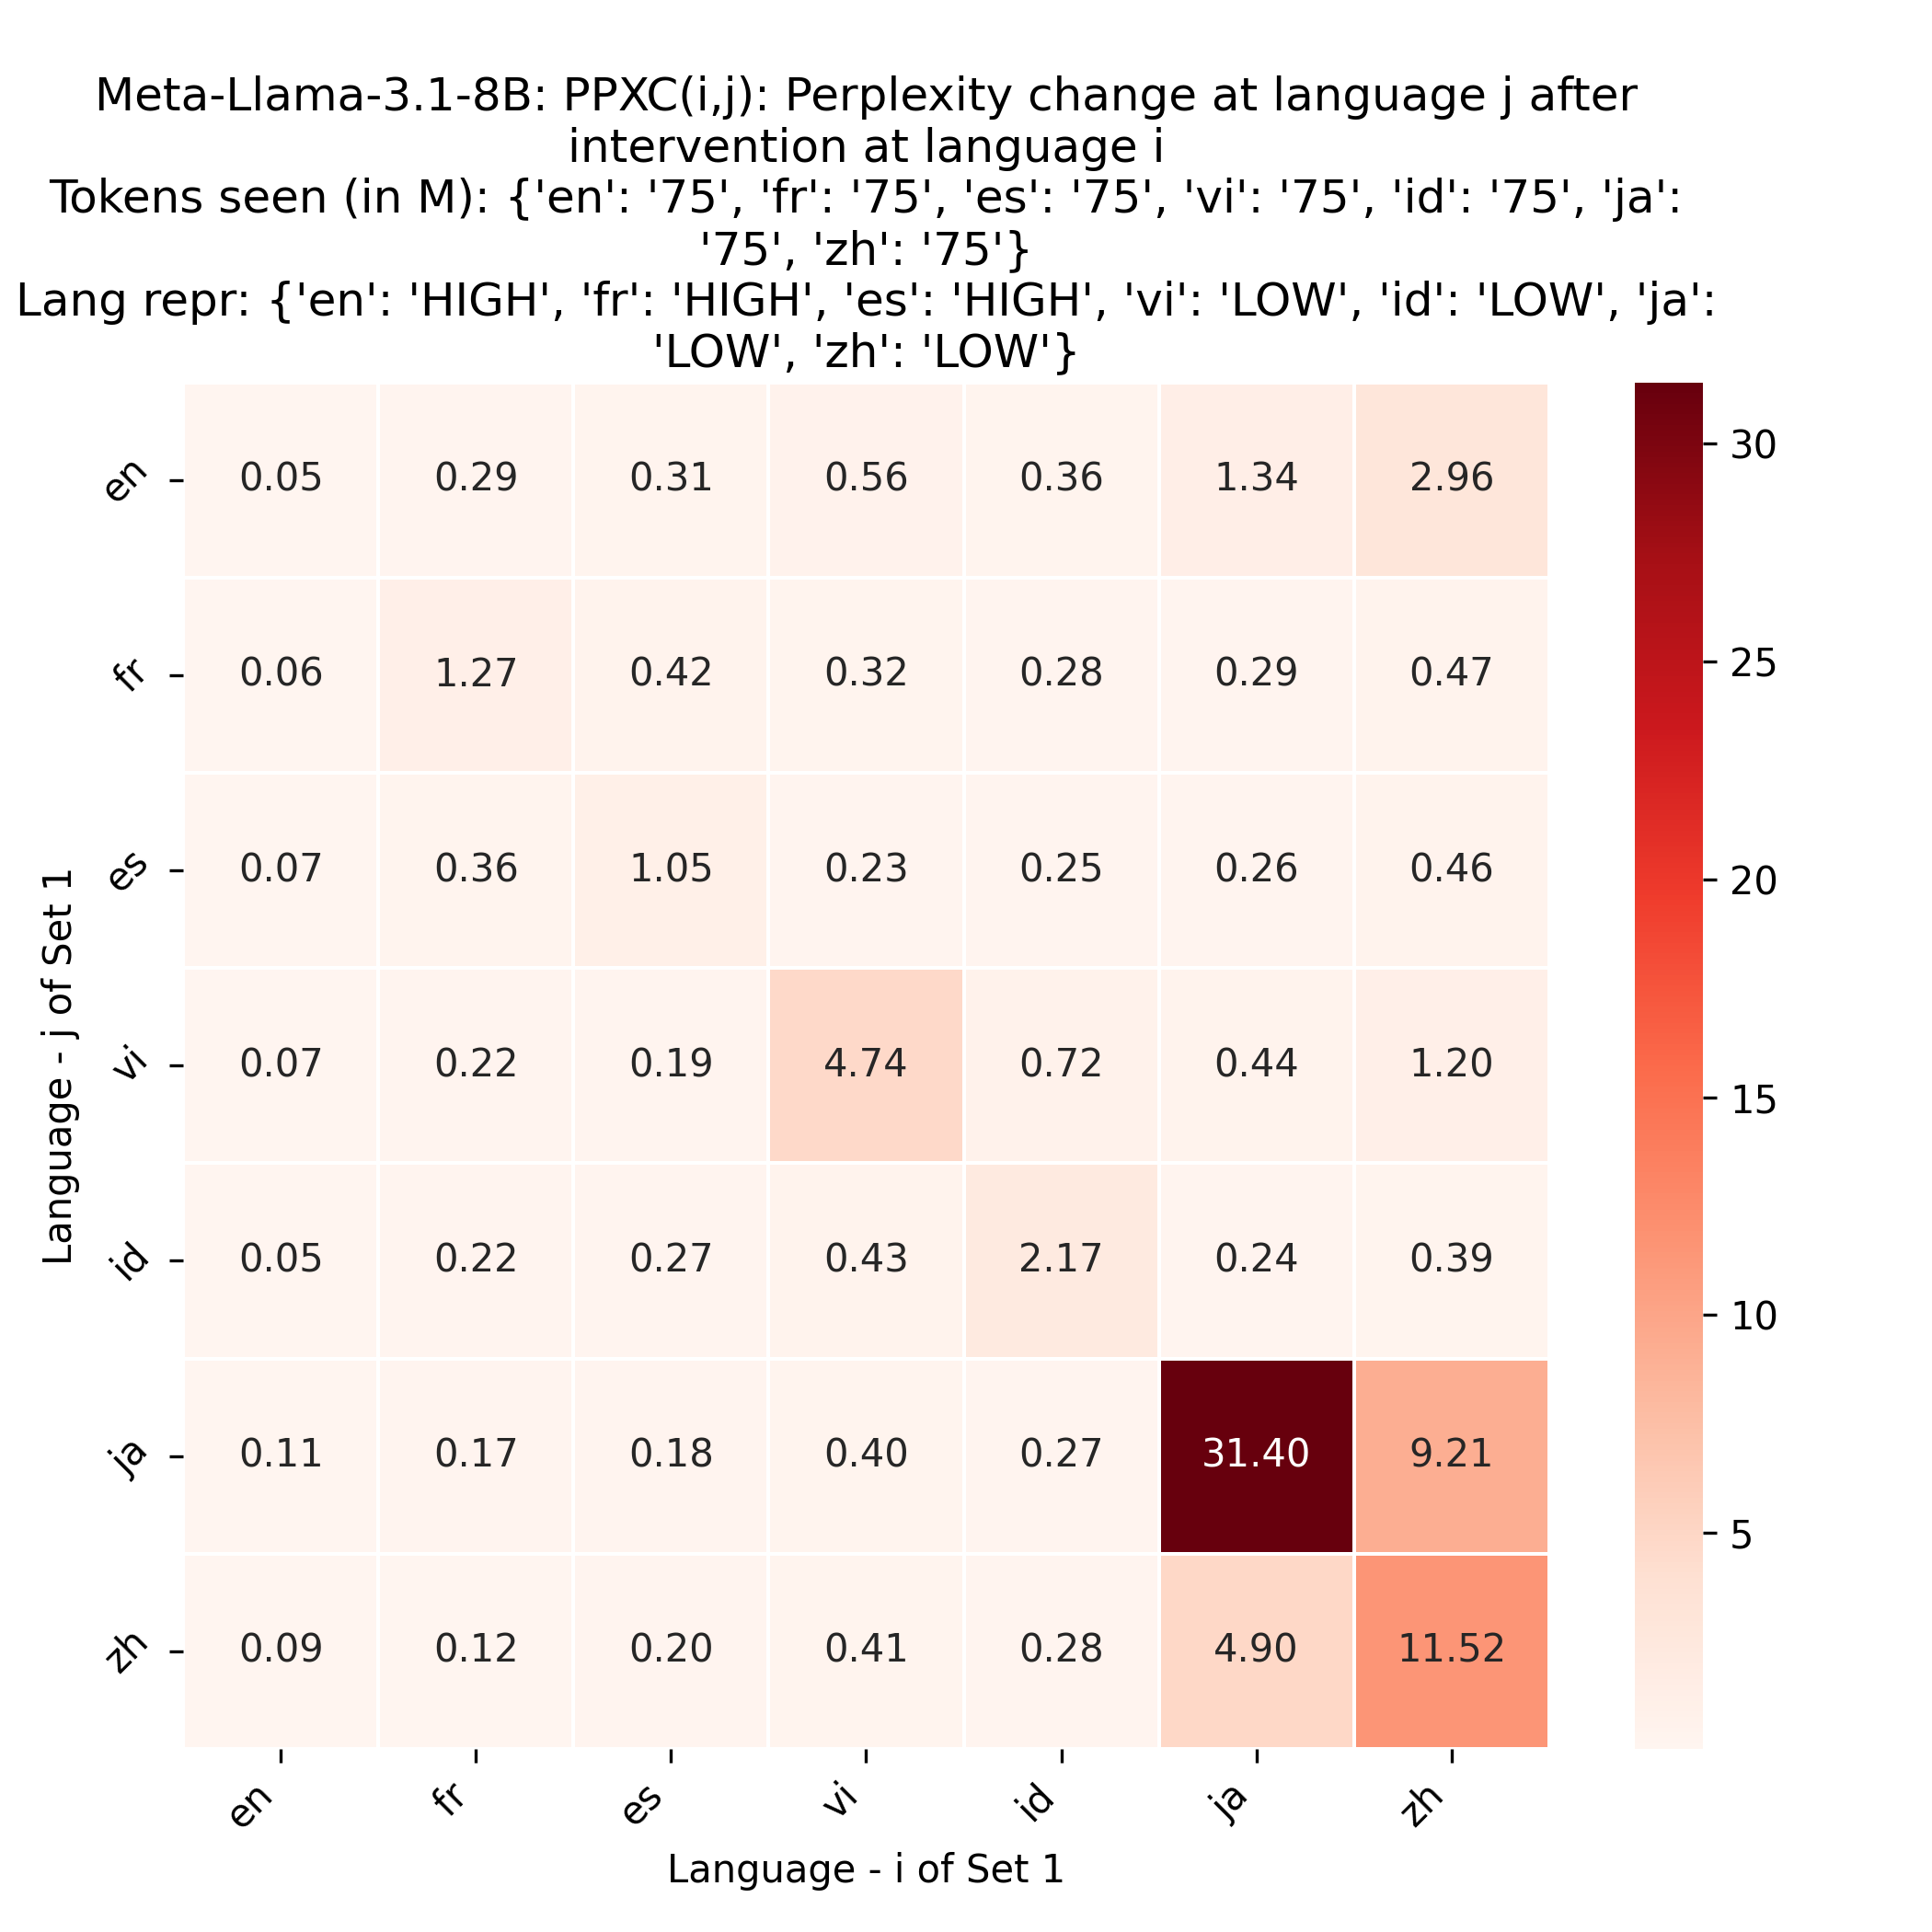
\includegraphics[width=0.45\textwidth]{Chapters/Chapter_5/perplexity/Meta-Llama-3.1-8B/set1/ppx_change.png} &
		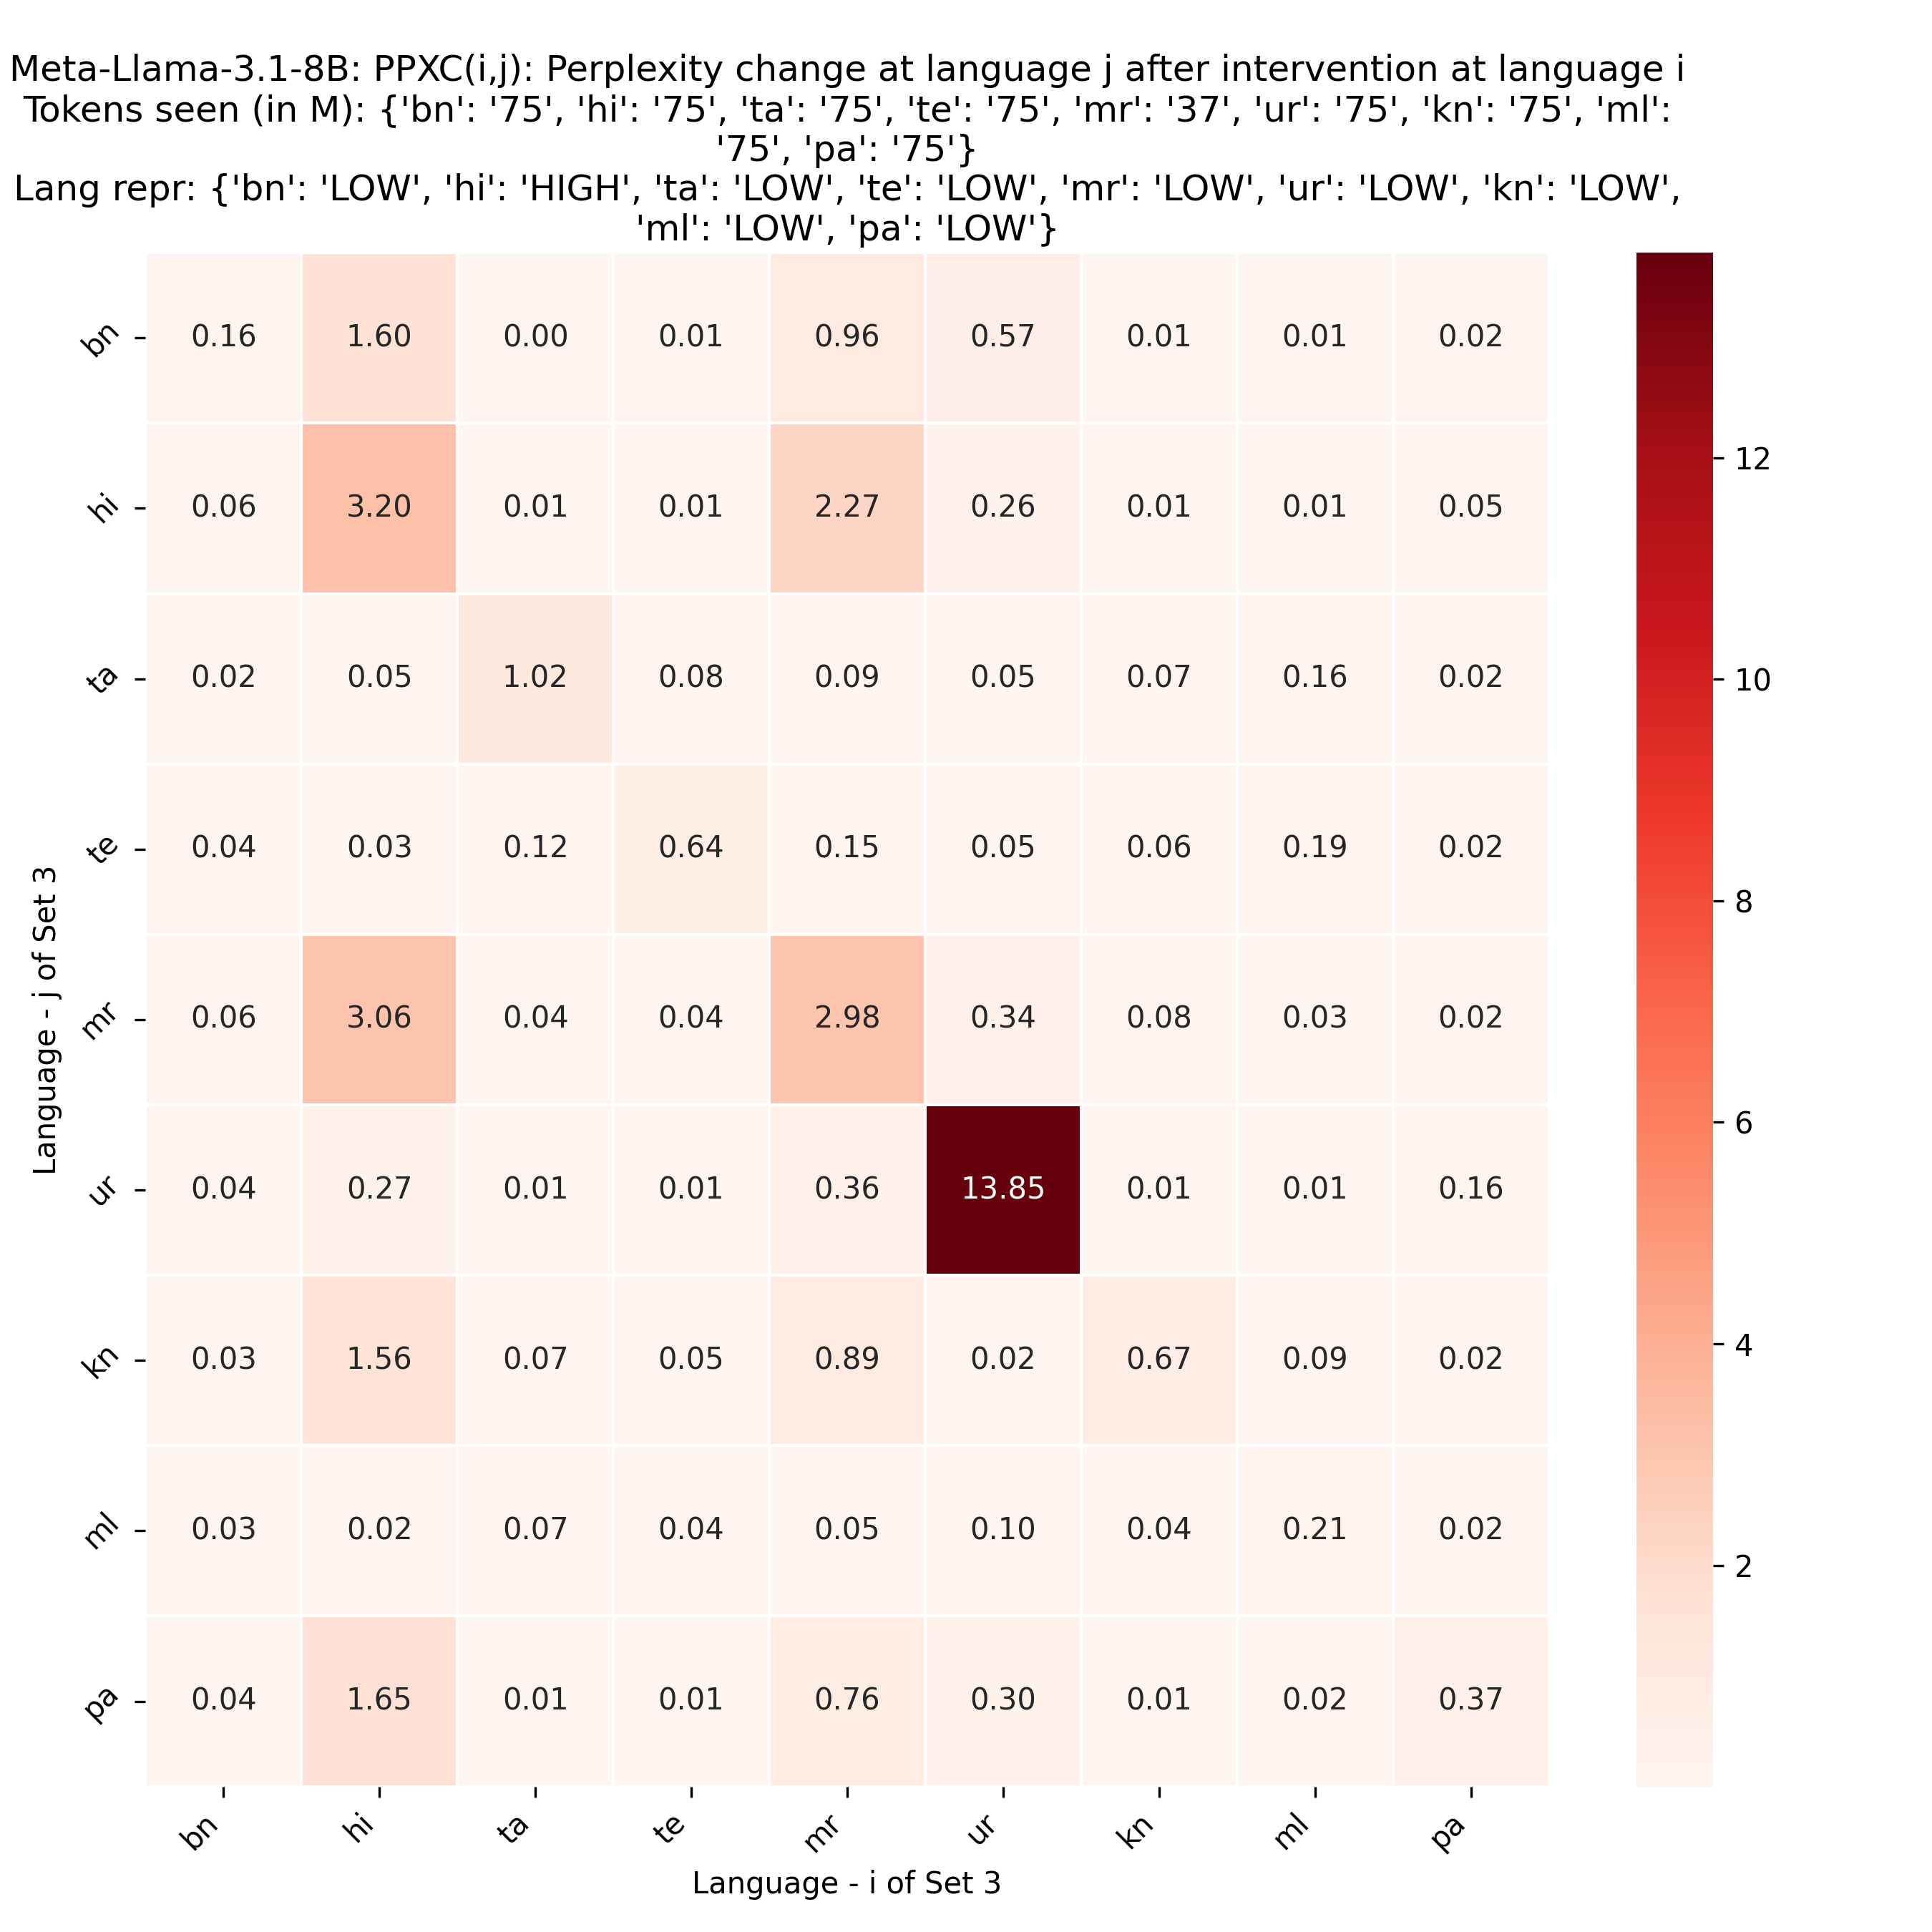
\includegraphics[width=0.45\textwidth]{Chapters/Chapter_5/perplexity/Meta-Llama-3.1-8B/set3/ppx_change.png} \\
		\textbf{Set1: Perplexity Change} &
		\textbf{Set3: Perplexity Change}
	\end{tabular}
	\caption{Perplexity change $\text{PPXC}(i,j)$ for LAPE method for Set1 and Set3.}
	\label{fig:ppx_change}
\end{figure}

From Figure \ref{fig:ppx_change}, we observe the following key trends:
\begin{itemize}
	\item For \textbf{Set1}, interventions at low-resource languages such as \textit{ja} lead to substantial perplexity changes for other low-resource languages (\textit{zh, id, vi}), as indicated by high $\text{PPXC}(i,j)$ values. This suggests that these languages share overlapping representations in the model.
	\item For \textbf{Set3}, interventions at \textit{ur} result in significant perplexity changes for other low-resource languages like \textit{ta, te}, highlighting the influence of high-representation languages on their low-representation counterparts.
\end{itemize}

\subsection{XNLI Task Results After Targeted Neurons Fine-Tuning}

Table~\ref{tab:xnli_results} summarizes the results of the fine-tuning experiments on the XNLI task. These experiments involve evaluating the zero-shot performance of the model on Vietnamese (\textit{vi}), Hindi (\textit{hi}), and Urdu (\textit{ur}) after targeted neuron fine-tuning and statistical interventions. The table reports the results (\textit{No Int}) alongside the effects of interventions using statistical patterns (\textit{Mean}, P75, P90, and P95).

\textbf{Insights from Results:}
\begin{itemize}
	\item \textbf{No Intervention Performance:} The model (\textit{No Int}) achieves robust zero-shot performance for all three languages. For instance, in \textit{vi}, the baseline accuracy is highest (0.8053) with no fine-tuning of neurons.
	\item \textbf{Impact of Interventions:} Statistical interventions generally degrade the model's performance. The degradation becomes more significant with higher percentiles (e.g., P90 and P95), indicating that extreme activation values may negatively affect generalization.
	\item \textbf{Language-Specific Trends:} For \textit{ur}, fine-tuning both English and Urdu neurons (\textit{set6\_en + ur}) shows marginal improvement in baseline performance compared to other setups. However, statistical interventions still result in performance drops.
	\item \textbf{Fine-Tuning Trade-Offs:} Fine-tuning neurons specific to the target language (\textit{set1\_vi, set6\_hi, set6\_ur}) offers better specialization for the target language. However, this comes at the cost of reduced generalization, as seen in the reduced accuracy for higher percentiles.
\end{itemize}

\begin{table}[ht]
	\centering
	\renewcommand{\arraystretch}{1.3}
	\setlength{\tabcolsep}{4pt}
	\begin{tabularx}{\textwidth}{|X|X|X|X|X|X|X|}
		\hline
		\textbf{Fine-tune Neurons} & \textbf{Eval Lang} & \textbf{No Int} & \textbf{Int by $\mu$} & \textbf{Int by P75} & \textbf{Int by P90} & \textbf{Int by P95} \\
		\hline
		null & vi & 0.8053 & 0.7955 & 0.7915 & 0.7903 & 0.7897 \\
		set1\_en & vi & 0.8017 & 0.7957 & 0.7867 & 0.7847 & 0.7847 \\
		set1\_vi & vi & 0.8007 & 0.7951 & 0.7881 & 0.7855 & 0.7845 \\
		set1\_en+vi & vi & 0.8009 & 0.7943 & 0.7865 & 0.7845 & 0.7833 \\
		\hline
		null & hi & 0.7501 & 0.7521 & 0.7496 & 0.7499 & 0.7506 \\
		set1\_en & hi & 0.7476 & 0.7456 & 0.7454 & 0.7448 & 0.7434 \\
		set6\_en & hi & 0.7491 & 0.7456 & 0.7464 & 0.7458 & 0.7441 \\
		set6\_hi & hi & 0.7492 & 0.7456 & 0.7461 & 0.7448 & 0.7431 \\
		set6\_en+hi & hi & 0.7488 & 0.7448 & 0.7451 & 0.7446 & 0.7431 \\
		\hline
		null & ur & 0.7002 & 0.7044 & 0.7028 & 0.6938 & 0.6904 \\
		set6\_en & ur & 0.6984 & 0.7041 & 0.7026 & 0.6964 & 0.6923 \\
		set6\_ur & ur & 0.6984 & 0.7054 & 0.7024 & 0.6952 & 0.6913 \\
		set6\_en+ur & ur & 0.6992 & 0.7061 & 0.7021 & 0.6954 & 0.6919 \\
		\hline
	\end{tabularx}
	\caption{XNLI task results after targeted neurons fine-tuning for LAPE method. The training language is always English.}
	\label{tab:xnli_results}
\end{table}

The results highlight the complexities of fine-tuning specific neurons for multilingual tasks. While targeted fine-tuning can improve certain aspects of language specialization, it often comes at the cost of generalization.


















\section{Activation Probability 90p Experiments}

\subsection{Language Neuron Distribution}

In this section, we analyze the distribution of language-specific neurons across the selected languages: \textit{en}, \textit{vi}, \textit{hi}, and \textit{ur}. Unlike LAPE, this approach is set-independent, meaning the results remain consistent regardless of the set of languages considered. Each language has the same number of neurons, precisely 573, allocated based on 0.0125\% of the total number of neurons. This ensures fairness and uniformity in the analysis across different languages. The emphasis here is on examining the overlap and layer-wise distribution of these neurons. The overlap matrix, as shown in Figure~\ref{fig:combined_lang_neurons}, highlights the extent to which neurons are shared between languages. This indicates that while there is some degree of shared representation, the neurons largely retain their language specificity.

The layer-wise neuron distribution, depicted in Figure~\ref{fig:combined_lang_neurons}, provides insights into the depth at which language-specific features are encoded. For all languages, a significant concentration of neurons is observed in the lower layers (e.g., Layers 4–8). This suggests that fundamental linguistic features, such as syntax and basic semantics, are predominantly captured in the initial layers. In contrast, the middle and upper layers contain fewer language-specific neurons, indicating that these layers might focus more on higher-level abstractions or tasks that are less language-dependent.


\begin{figure}[ht]
	\centering
	\begin{tabular}{cc}
		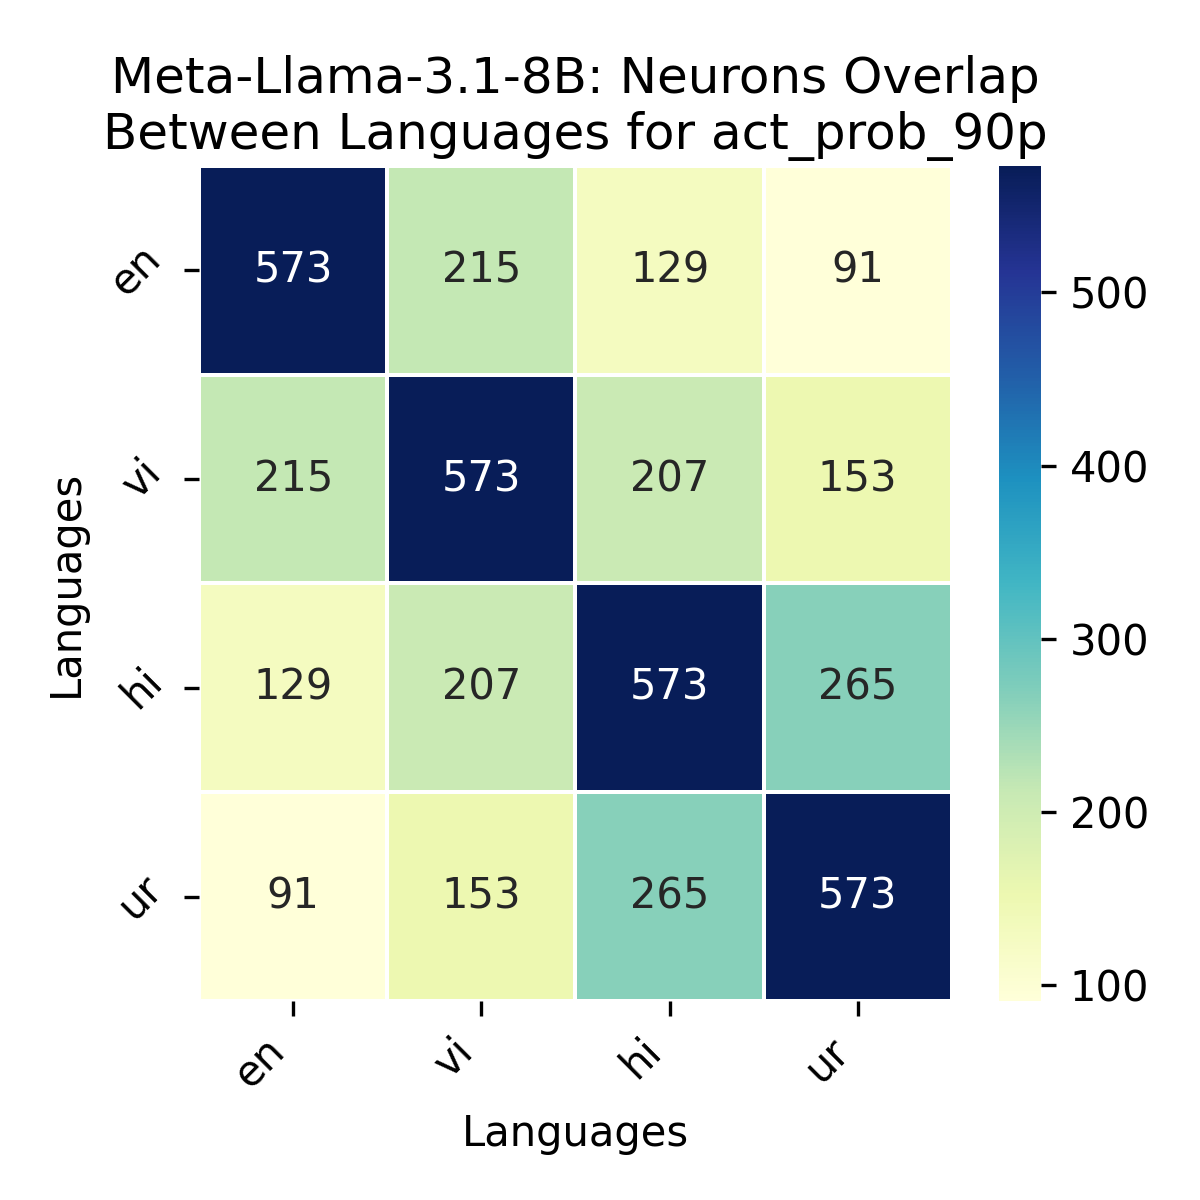
\includegraphics[width=0.60\textwidth]{Chapters/Chapter_5/lang_neurons/Meta-Llama-3.1-8B/act_prob_90p/lang_neurons_overlap.png} &
		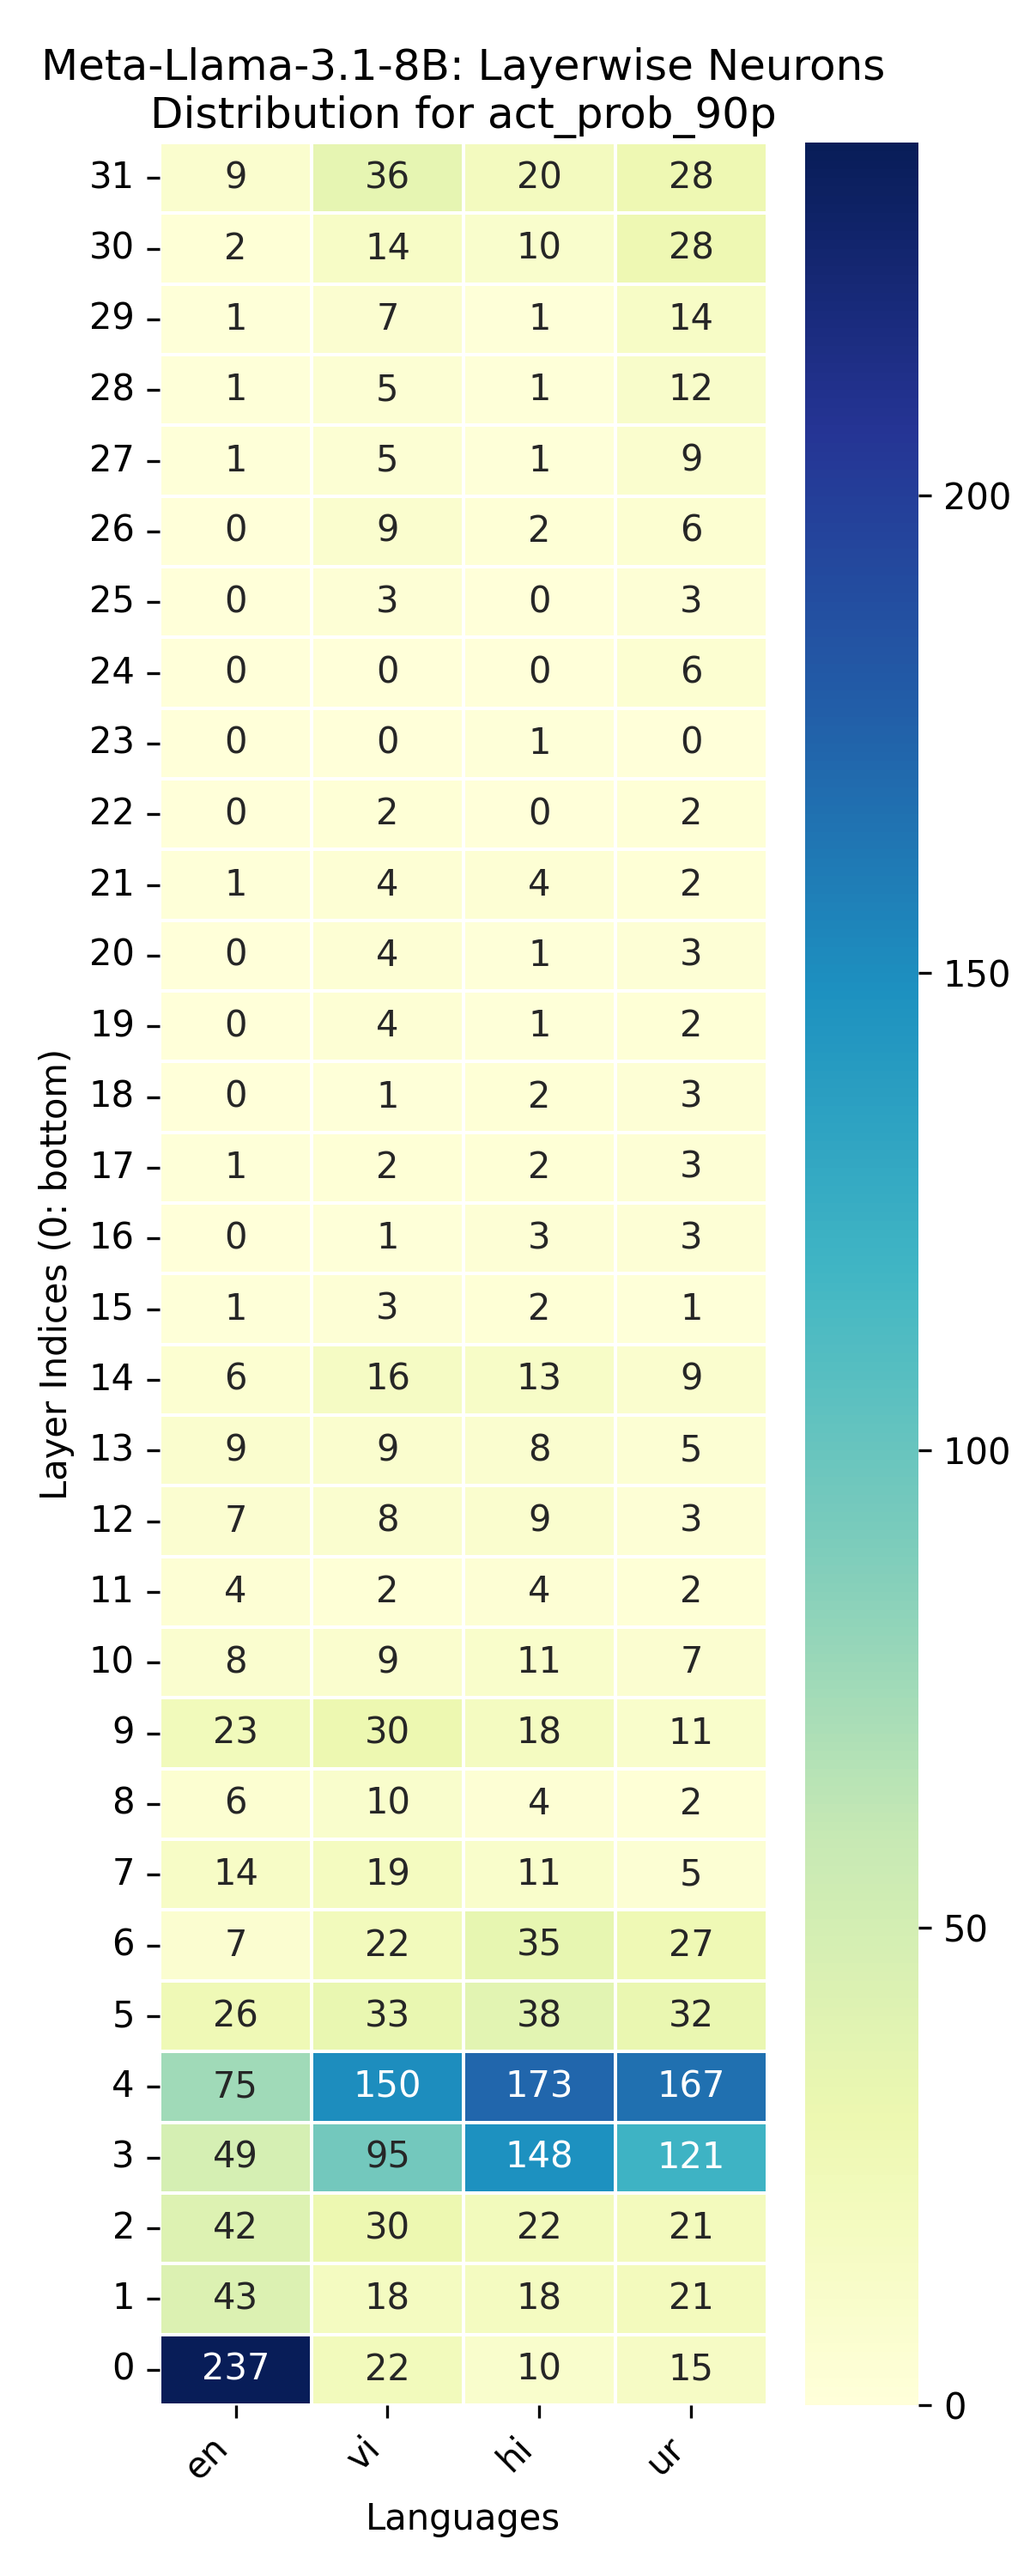
\includegraphics[width=0.30\textwidth]{Chapters/Chapter_5/lang_neurons/Meta-Llama-3.1-8B/act_prob_90p/layerwise_lang_neurons_dist.png} \\
		\textbf{Overlap Between Neurons} &
		\textbf{Layer-wise Neuron Dist}
	\end{tabular}
	\caption{Overlap between neurons and layer-wise neurons distribution for activation probability 90p method.}
	\label{fig:combined_lang_neurons}
\end{figure}


This method demonstrates a significant advantage over LAPE as it ensures consistency and fairness across languages. Since the language-specific neurons are determined independently of the set of languages considered, the analysis does not suffer from the set-dependent biases inherent in LAPE.

\subsection{Perplexity Change}

The experimental results for the perplexity change (\textit{PPXC}) are presented in this section. These results focus on analyzing the impact of interventions at one language (\textit{i}) on the perplexity of another language (\textit{j}) within the same experimental setup. The datasets used for these computations are derived from the Wikipedia corpus for the respective languages.

\begin{figure}[ht]
	\centering
	\begin{tabular}{cc}
		% First Figure: act_prob_zero
		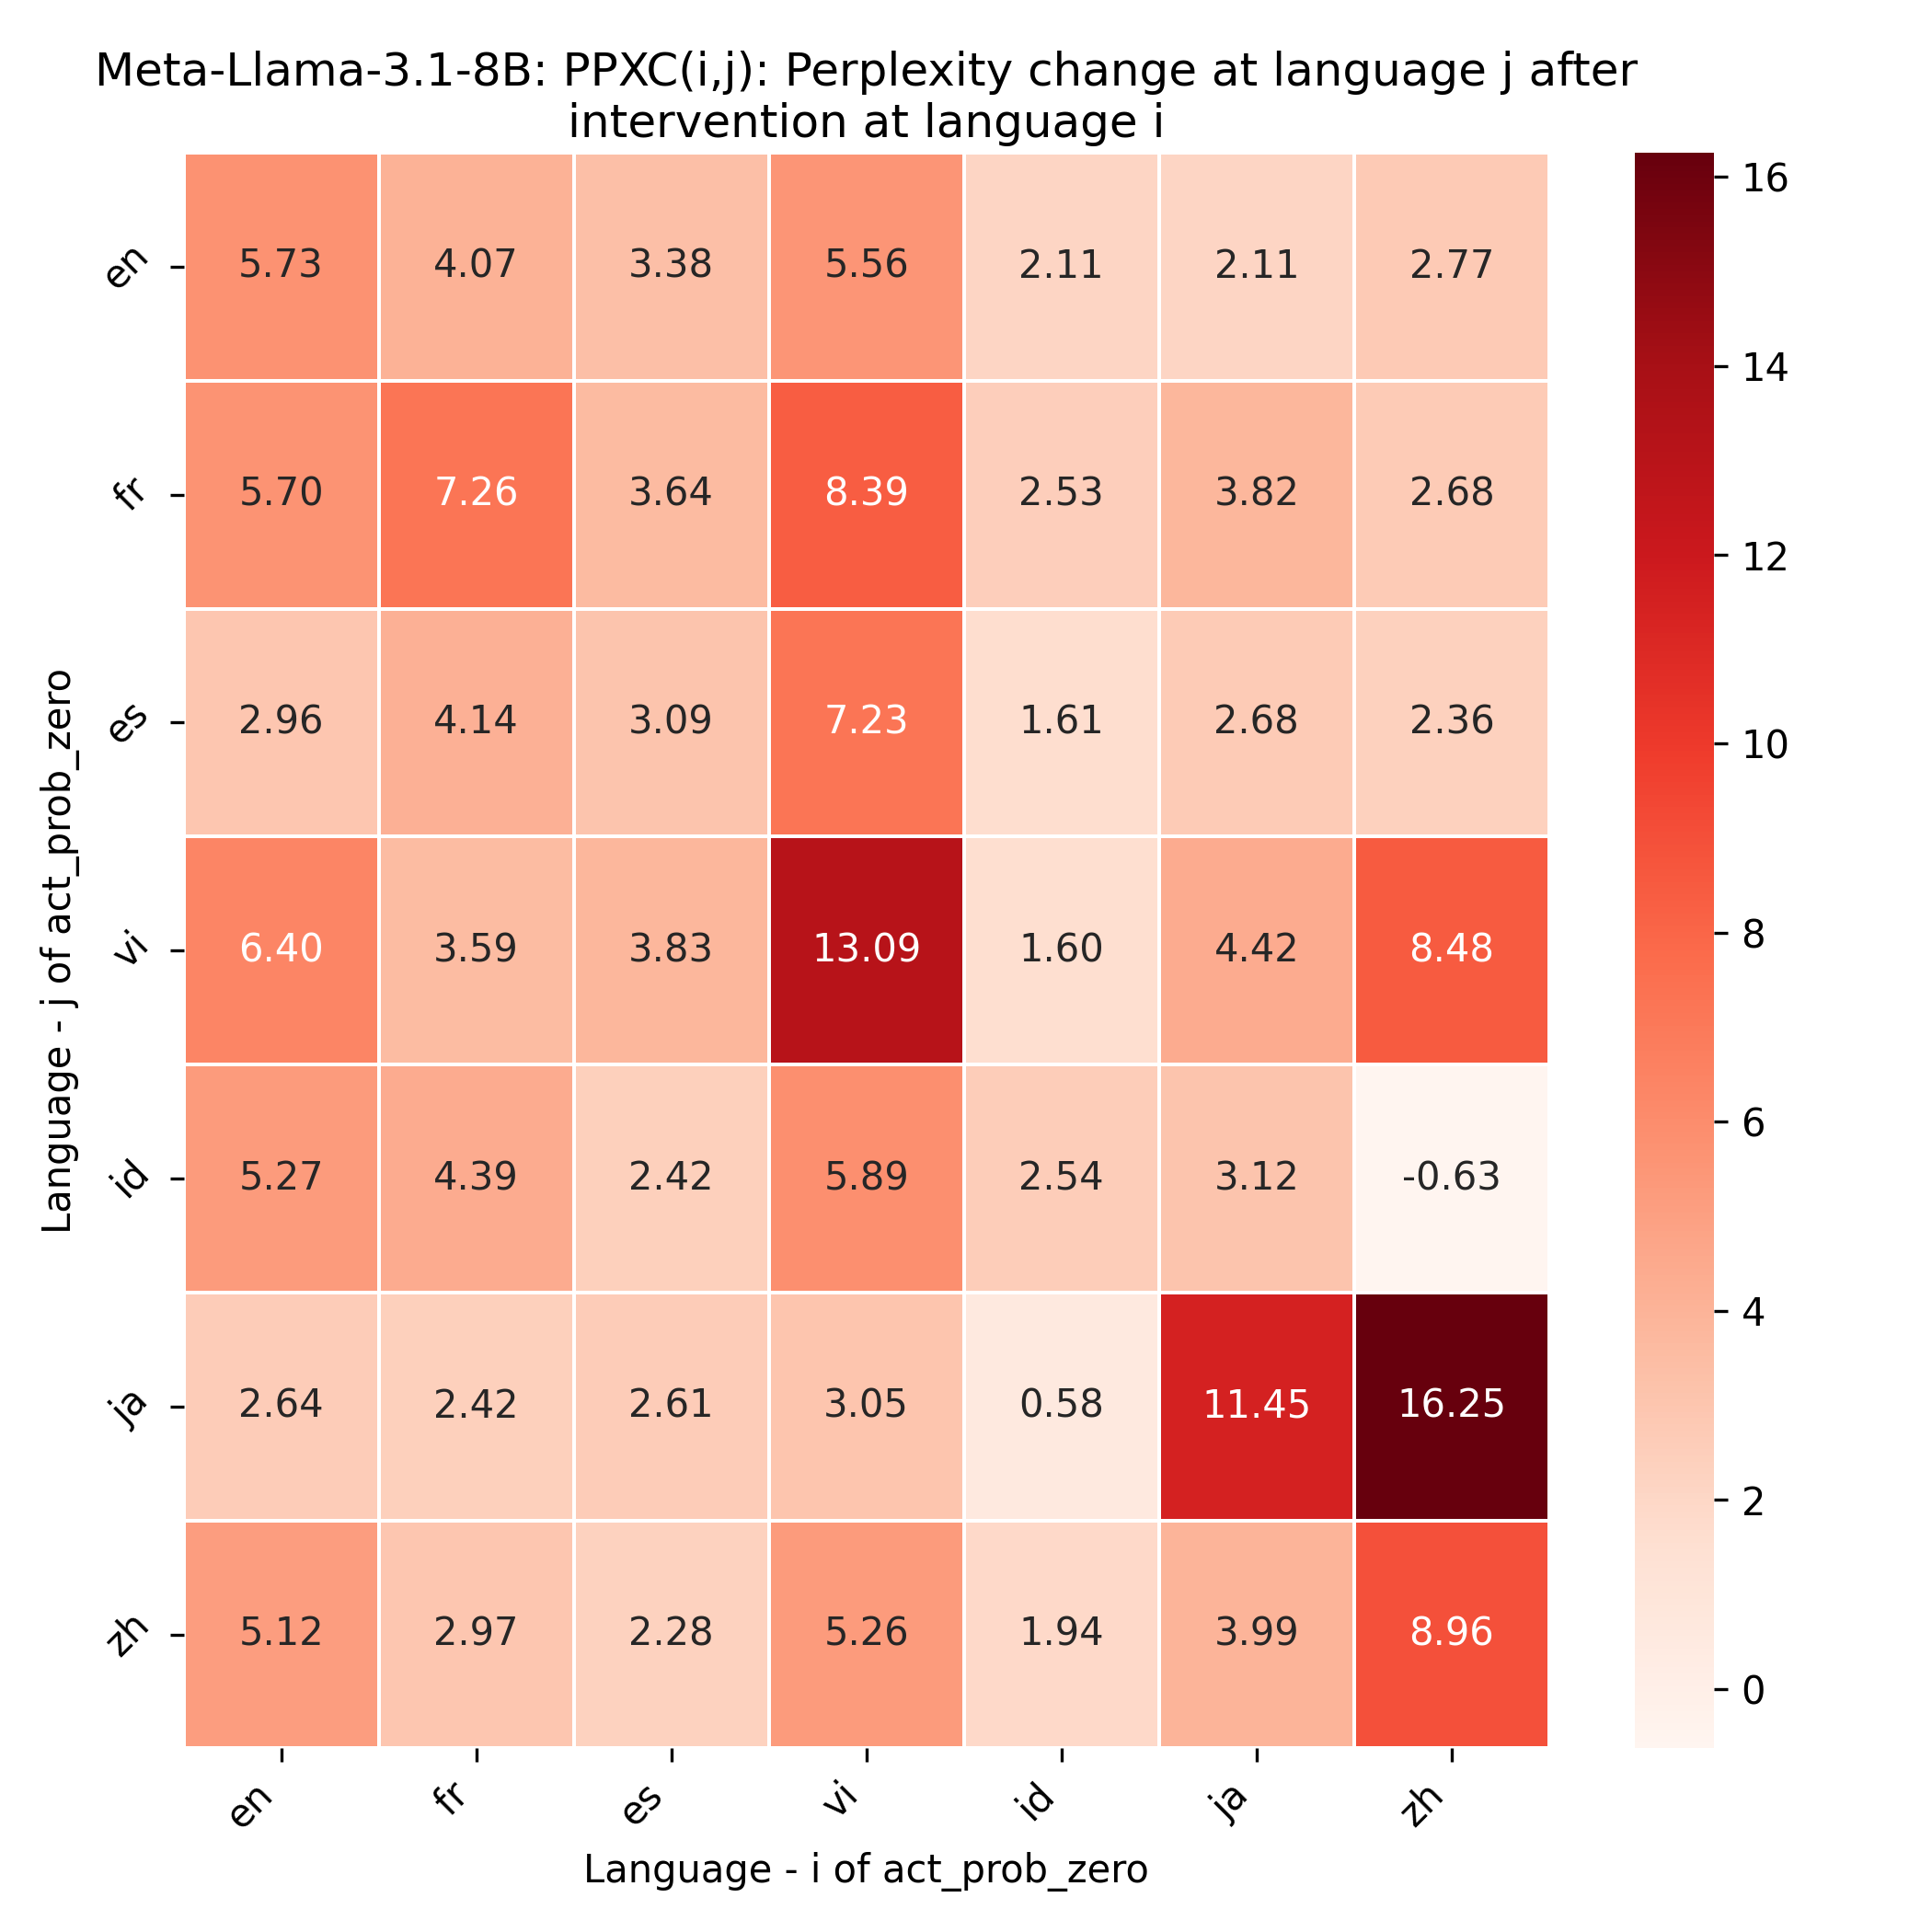
\includegraphics[width=0.45\textwidth]{Chapters/Chapter_5/perplexity/Meta-Llama-3.1-8B/act_prob_zero/ppx_change.png} &
		% Second Figure: act_prob_90p
		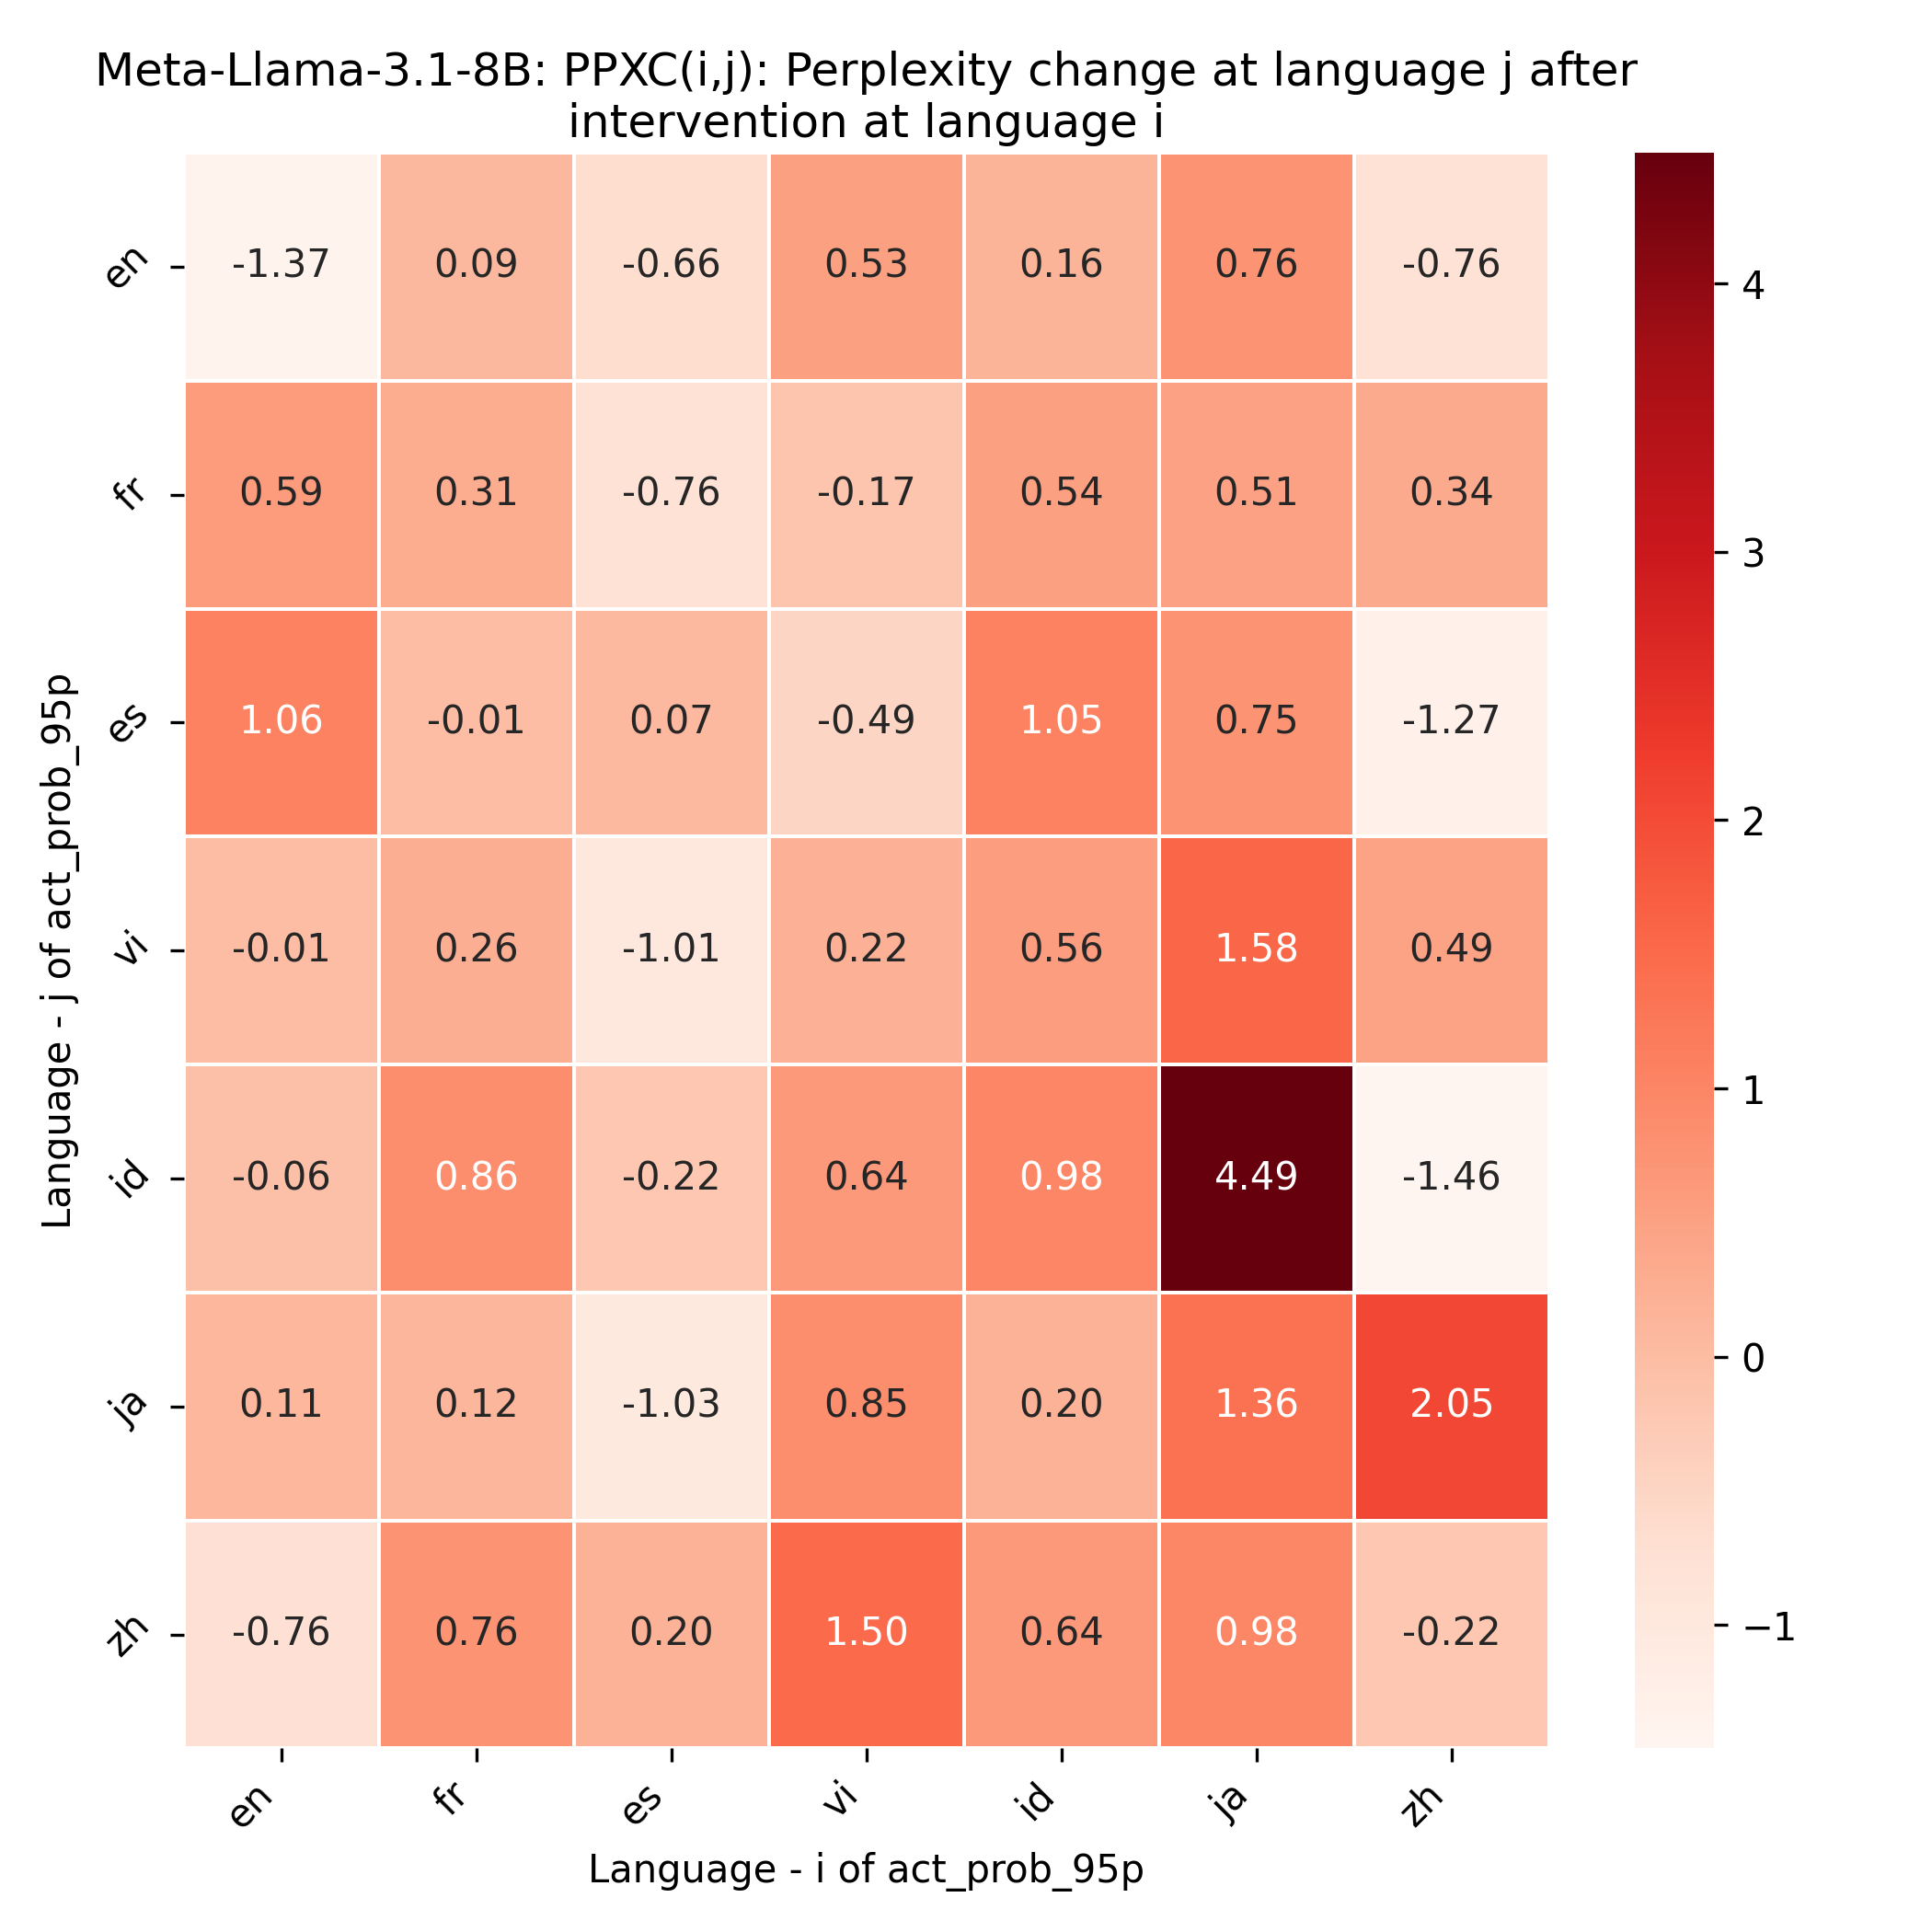
\includegraphics[width=0.45\textwidth]{Chapters/Chapter_5/perplexity/Meta-Llama-3.1-8B/act_prob_95p/ppx_change.png} \\
		\textbf{(a) PPXC for act\_prob\_zero} & \textbf{(b) PPXC for act\_prob\_90p}
	\end{tabular}
	\caption{Perplexity change $\text{PPXC}(i,j)$ for activation probability based methods.}
	\label{fig:ppxc_results}
\end{figure}

\textbf{Analysis:} From Figure \ref{fig:ppxc_results}, the following insights can be drawn:
\begin{itemize}
	\item \textbf{Non-Diagonal Behavior:} The perplexity change values are not strictly diagonal, indicating that interventions in one language (\textit{i}) can significantly influence the perplexity of another language (\textit{j}). This behavior suggests a complex interplay between the language representations within the model, where neurons may encode shared features across multiple languages.
	
	\item \textbf{Negative Values:} In some cases, the perplexity change values are negative, implying that deactivating certain neurons in one language can paradoxically improve the language capability of another. This counterintuitive result highlights the possibility that some neurons may act as bottlenecks, restricting the efficient representation of linguistic features in other languages.
	
	\item \textbf{Further Analysis Required:} The exact mechanisms underlying these phenomena are unclear and require further exploration. Factors such as the resource level of the languages, the layer-wise distribution of neurons, and the training dynamics of shared representations could play a critical role.
\end{itemize}










